\documentclass{article}

\usepackage[english]{babel}
\usepackage[utf8]{inputenc}

% define document margins
\usepackage[top=30mm, bottom=30mm, right=30mm, left=30mm]{geometry}

% packages to allow for mathematical expressions / fonts / proofs
\usepackage{amsmath}
\usepackage{amsfonts}
\usepackage{amsthm}
% package to include graphics
\usepackage{graphicx}
% pachakge to wrap figures into text
\usepackage{wrapfig}

\usepackage{hyperref}
% package to use float options such as H in defining the position of a figure
\usepackage{float}
% package to indent the first paragraph in each section
\usepackage{indentfirst}

\title{
  N-Units Away Curves
}
\date{
  March 28, 2020
}
\author{
  Orion Haunstrup \\
  University of Rochester \\
  \href{mailto:orioning@gmail.com}{orioning@gmail.com}
}

\begin{document}

  \maketitle

  \section{Introduction}

This paper will examine a mathematics theory I’ve been working on for quite some time. I call it the study of ``$N$-Units Away Curves''. I actually first discovered this fascinating little enigma in my doodles when I was perhaps only five or six years old. The particular little geometric phenomenon I discovered was really interesting, and I couldn’t explain it at the time. All these years later as a grown man and mathematician, it gives me a nice feeling of catharsis to finally rigorously address this question and comprehend its mysteries.

% define a variable w for the width of the section for a figure
\newcommand\w{.40\linewidth}
% define a variable fw for the width of a figure with respect to the line its in
\newcommand\fw{.90\textwidth}

\begin{figure}[H] % [H]: insert the figure 'here!', in this position in the code, overriding compiler preferences
  \centering % center the set of figures with the respect to the page
  \begin{minipage}[b]{\w} % begin a section for one figure
    \centering % center one figure with respect to its section
    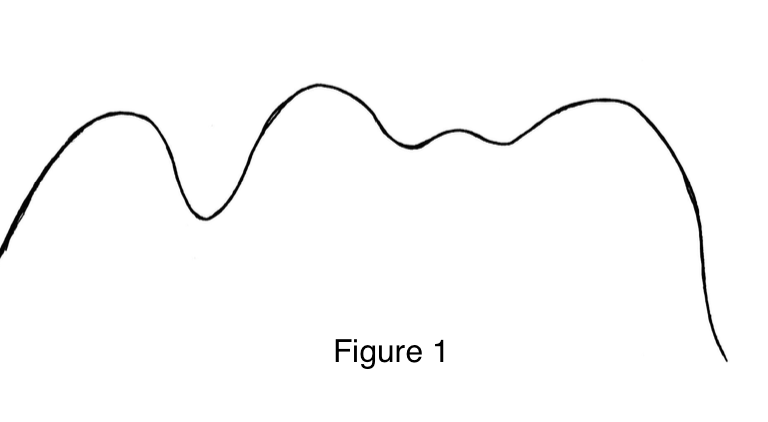
\includegraphics[width=\fw]{img/01-intro/01.png}
    \caption{A squiggle}
    \vspace{4ex}
  \end{minipage} % end
  \begin{minipage}[b]{\w}
    \centering
    \label{intro:2}
    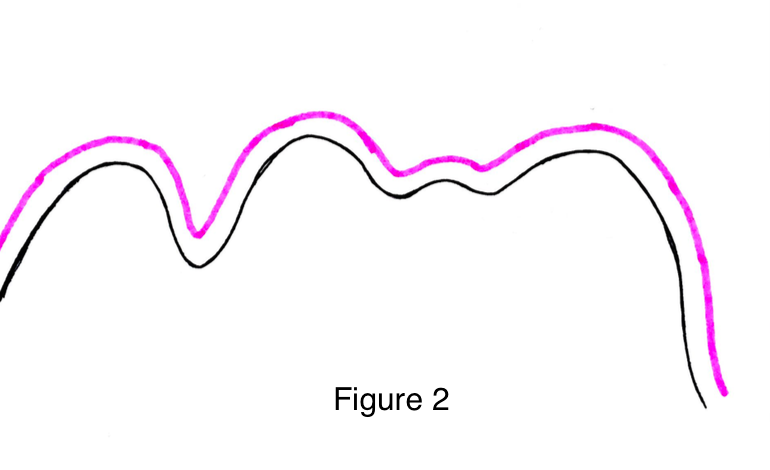
\includegraphics[width=\fw]{img/01-intro/02.png}
    \caption{Caption}
    \vspace{4ex}
  \end{minipage} % end
  \begin{minipage}[b]{\w}
    \centering
    \label{intro:3}
    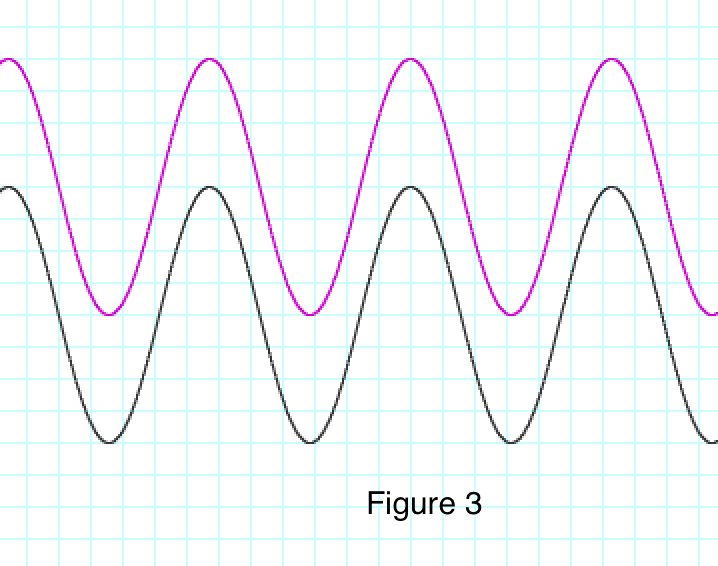
\includegraphics[width=\fw]{img/01-intro/03.png}
    \caption{Caption}
    \vspace{4ex}
  \end{minipage} % end
  \begin{minipage}[b]{\w}
    \centering
    \label{intro:4}
    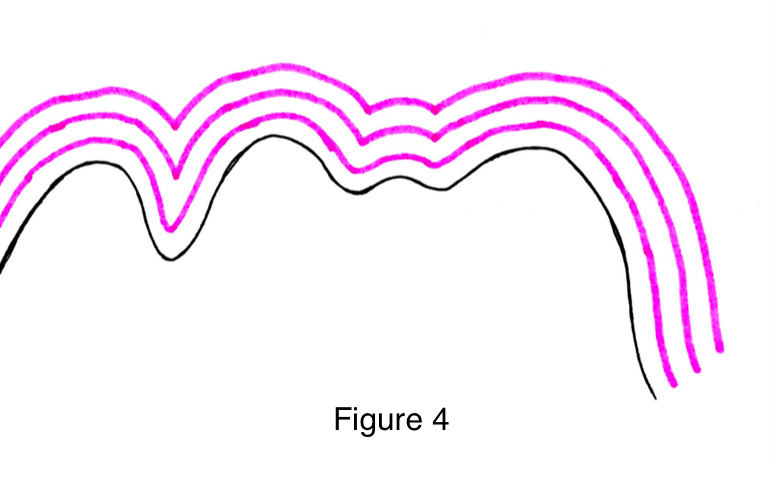
\includegraphics[width=\fw]{img/01-intro/04.png}
    \caption{Caption}
    \vspace{4ex}
  \end{minipage} % end
\end{figure}

As a little kid I discovered the following phenomenon in my doodles... Draw a curve. Any curve. A squiggle on a page will suffice. An example is provided in Figure $\ref{intro:1}$. It felt natural as a little kid to then draw another curve next to it that was the same distance away from the first at all points. (Fig $\ref{intro:2}$) Note that this is very different than what is more typically encountered in mathematics: two curves like $y = sin(4x)$ and $y = sin(4x) + 1$ are such that the second curve always remains 1 unit away from the first specifically in the $y$-direction (Fig $\ref{intro:3}$)... This is not what my little kid self meant at all. Imagine rolling a marble through the little ``tube'' that lies between $y = sin(4x)$ and $y = sin(4x) + 1$. At some points the little tube is wide and fat, at other points the tube gets very skinny and narrow. This is fundamentally different from the idea my kid self wanted us to do which was to take a curve and draw a $2^{nd}$ one next to it that would create a perfect nice little tube... a tube with the same diameter at all spots (see Figure $\ref{intro:2}$).

As a child doodling, it seemed natural to then repeat the process and draw another curve that lay the same distance away from this new curve. I’d repeat the process a whole bunch of times (Fig $\ref{intro:4}$), but then something curious always happened. I had started with a smooth curve. But as I ran the process again and again, inevitably the curves always ``got pointy.'' At first I assumed this was due to inaccuracies in my drawings, so I set out (crayons in hand) to draw these curves very accurately and was absolutely flabbergasted to discover that the phenomenon remained! What in the world was the reason for that? Why were the curves ``getting pointy''? A mystery was born. Many years passed by, and eventually I found myself enrolled in a high school Calculus class. One day we learned about inverse trigonometric functions (specifically) and a little while later it dawned on me... I finally had the mathematical tools I needed to further study these ``curves that lie $N$ units away''! My intent was now to figure out how to program my Pacific Tech Graphing Calculator to be able to take in an arbitrary function $y = f(x)$ and graph the associated curve that lies exactly $N$ units away at all points. I wanted to be able to finally see exactly what these curves looked like. I did so in the following manner.

  % define some variables
\newcommand\f{ f'(x_o) }
\newcommand\mfrac{ \dfrac{N}{|\f|} \f }
\newcommand\ang{ tan^{-1} \left( -\dfrac{1}{\f} \right) }
\newcommand\mcos{ cos \left( \ang \right) }
\newcommand\msin{ sin \left( \ang \right) }

% defining a new command for possible future use
\newcommand{\firstFormula}{

  \begin{equation} \tag{1} %  hard-set the number of this formula to be 1
    f_N(t) =
    \begin{bmatrix}
      x_N(t) \\
      y_N(t)
    \end{bmatrix} =
    \begin{cases}
      % case 1: f'(t) is non-0
      % expression
      \begin{bmatrix} % \mfrac, \ang, \mcos, \msin are defined above
        t - \mfrac \mcos \\
        f(t) + \mfrac \msin
      \end{bmatrix}, &
      % condition
      t \ni f'(t) \neq 0 \\
      % case 2: f'(t) is 0
      % expression
      \begin{bmatrix}
        t \\
        f(t) + N
      \end{bmatrix}, &
      % condition
      t \ni f'(t) = 0
    \end{cases}
  \end{equation}

}

\section{A First Formula}

Let $f: \mathbb{R} \to \mathbb{R}$ be any arbitrary twice differentiable function whose second derivative $f''$
is continuous. These are the kinds of functions this paper we’ll use to establish the science of the $N$-Units Away Curves. While you can talk about the building of an $N$-Units Away Curve from a segment of a function (not on all of $\mathbb{R}$), it’s very similar and just not as interesting. Likewise you can also talk about making $N$-Units Away Curves for functions that are non-differentiable or discontinuous, but in that case things often get very nasty very quickly.

Take your function $y = f(x)$ and we're now going to re-express that same function as a parametric function in terms of a variable $t$: \begin{equation*}
  \begin{bmatrix}
    x(t) \\
    y(t)
  \end{bmatrix} =
  \begin{bmatrix}
    t \\
    f(t)
  \end{bmatrix}
\end{equation*}, where $t$ assumes all values $t \in (- \infty, \infty)$. Pick any value $t_o \in \mathbb{R}$. $t_o$ corresponds to one unique point on the original curve $y = f(x)$, specifically the point $(t_o , f(t_o ))$. Fix an $N \in \mathbb{R}$. To every one of these points we are going to construct an associated point that lies exactly $N$ units away in the direction of the normal line to the curve at that point. Let $x_o = t_o$ . It’s a basic Calc 1 fact that at $x = x_o$ , the slope of the normal line is $-\dfrac{1}{f'(x_o)}$, assuming $f'(x_o)$ is non-zero. We can use arctangent to convert from slope to degrees. We get that the angle from the positive $x$-axis to the normal line is $\ang$.

We can then use $cos(\theta)$ to convert this angle to an $x$-distance and $sin(\theta)$ to convert this angle to a $y$-distance. If we multiply these both by $N$ we can obtain a normal vector $\langle N \mcos, \allowbreak N \msin \rangle $ which is exactly $N$ units long and points in the direction of the normal line to the curve $y = f(x)$ at $x = x_o$. The only last issue that causes trouble is the issue of which way we are trying to travel on that normal line? Let’s define it such that when N is positive, we obtain points $N$ units away and above the curve $y = f(x)$, and when $N$ is negative, we obtain points $N$ units away and below the curve. When $f'(x_o)$ is negative, the normal vector stated above points up and to the right, so we’re fine. It points to a spot above the curve. When $f'(x_o)$ is positive however, the normal vector points down and to the right, so we must multiply the whole vector by -1. This resolves the issue. We arrive at the desired normal vector that points $N$ units away into the ``up'' direction along the normal line to $y = f(x)$ at $x = x_o$. That vector is $\langle - \mfrac \mcos, - \mfrac \msin \rangle$.

We can utilize this to derive a parametric formula for the $N$-Units Away Curve to $y = f(x)$
in all cases where $f'(x_o) \neq 0$. But what about when is equal to 0? It’s nice and simple then.
We simply move $N$ units along a perfectly vertical normal line.

Thus the formula for the $N$-Units Away Curve to $y = f(x)$ is:

\firstFormula

  \section{Some Examples}

Let’s take a moment to examine some examples of the fascinating new graphs I obtained! Each will display a number of $N$-Units Away Curves next to one another.

% see src/01-intro.tex for more extensive commented code of set of figures
\renewcommand\w{.40\linewidth}
\renewcommand\fw{.90\textwidth}

\begin{figure}[H]
  \centering
  \begin{minipage}[b]{\w}
    \centering
    \label{example:1}
    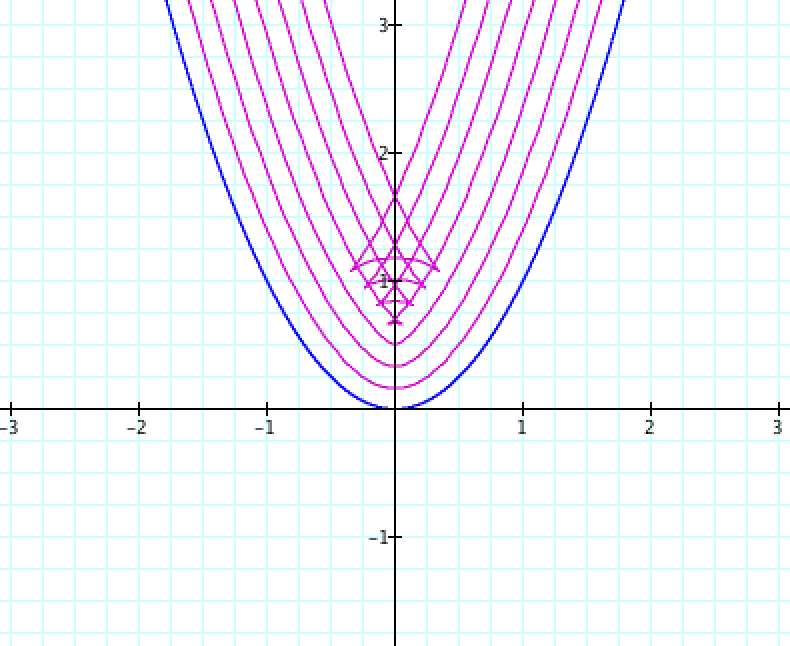
\includegraphics[width=\fw]{img/03-some-examples/01.png}
    \caption{$ f(x) = x ^ 2, N > 0 $}
    \vspace{4ex}
  \end{minipage} % end
  \begin{minipage}[b]{\w}
    \centering
    \label{example:2}
    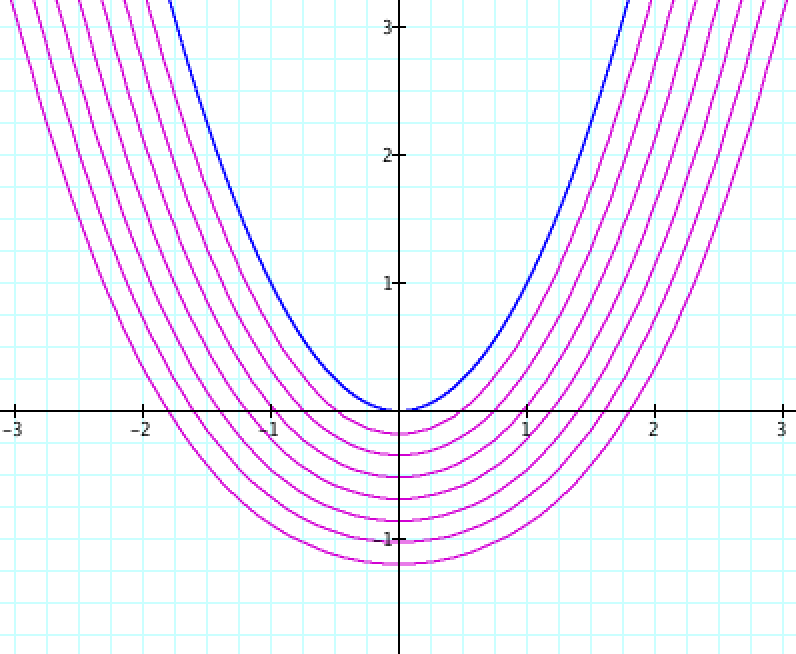
\includegraphics[width=\fw]{img/03-some-examples/02.png}
    \caption{$ f(x) = x ^ 2, N < 0 $}
    \vspace{4ex}
  \end{minipage} % end
\end{figure}

\renewcommand\w{.80\textwidth}

\begin{figure}[H]
  \label{example-2}
  \centering
  \begin{minipage}[b]{\w}
    \centering
    \label{example:3}
    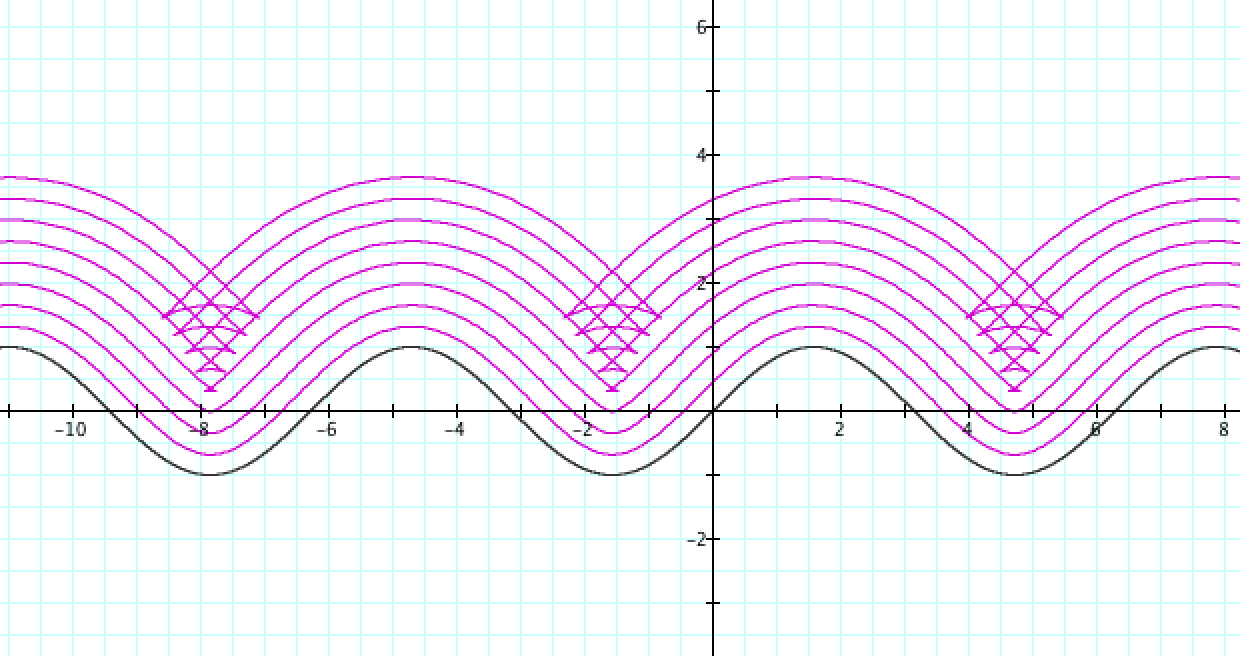
\includegraphics[width=\fw]{img/03-some-examples/03.png}
    \caption{$ f(x) = sin x, N > 0 $}
    \vspace{4ex}
  \end{minipage} % end
\end{figure}

\renewcommand\w{.40\textwidth}

\begin{figure}[h]
  \begin{minipage}[b]{\w}
    \centering
    \label{example:4}
    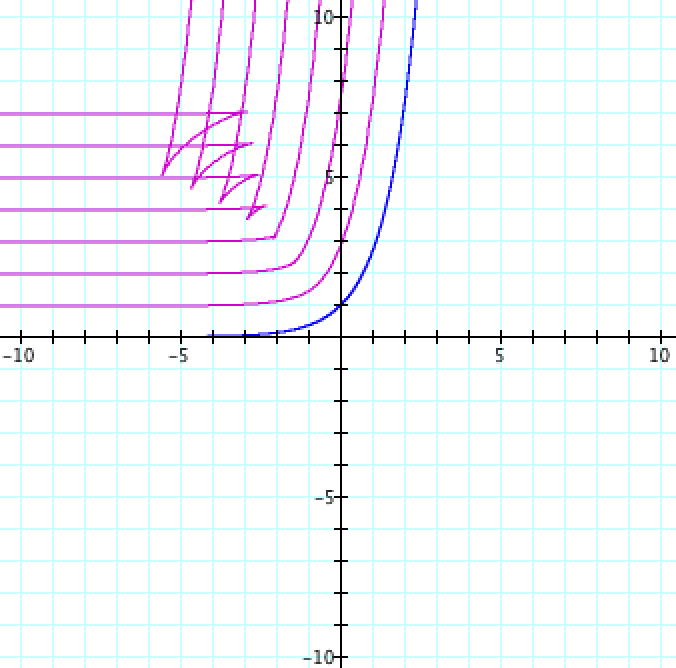
\includegraphics[width=\fw]{img/03-some-examples/04.png}
    \caption{$f(x) = e ^ x, N > 0$}
    \vspace{4ex}
  \end{minipage} % end
  \begin{minipage}[b]{0.5\linewidth}
    \centering
    \label{example:5}
    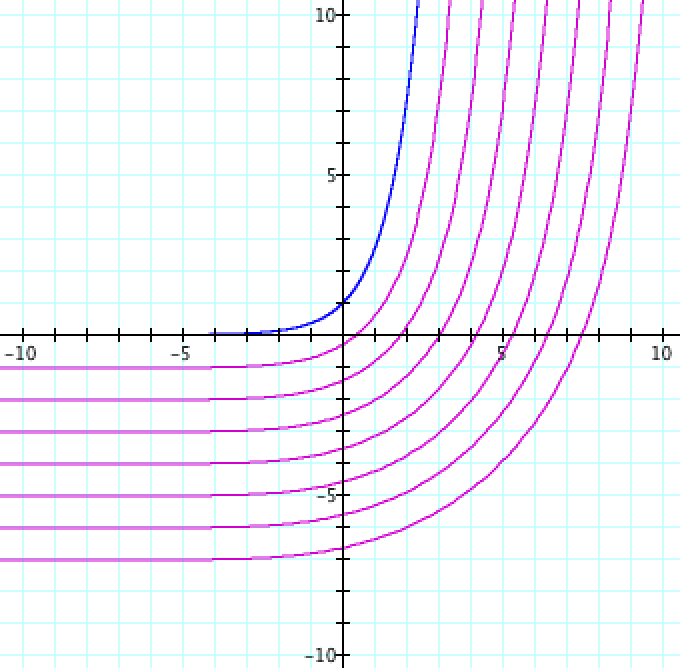
\includegraphics[width=\fw]{img/03-some-examples/05.png}
    \caption{$f(x) = e^x, N < 0$}
    \vspace{4ex}
  \end{minipage} % end
\end{figure}

I loved these graphs! After so many years of drawing these things by hand, it was great to finally see them exactly and perfectly produced by computer. Playing with these $N$-Units Away Curves, I noted a few patterns very quickly.

\begin{itemize}
    \item The curves seem to stay smooth if you push them out opposite to the direction that the curve is bending.
    \item On the other hand, when you push the curves into the direction that the curve is bending, they seem to inevitably reach a critical value of $N$ and then ``crunch'' upon themselves, ceasing thereafter to pass the vertical line test and even be a function at all.
    \item When you produce these graphs, set $N$ to zero, and observe what happens as you gradually increase $N$... you find that for each region of the curve that has any bend to it, at some critical value of $N$ the $N$-Units Away Curves seem to collapse and crunch upon themselves at a unique ``crunch spot''.
    \item Past that critical value, the $N$-Units Away Curves seem to thereafter generate a sort of odd-ball curvy triangle. These ``Divot Triangles'' were highly unexpected and I found them very intriguing. They always seemed to originate directly out of each crunch spot and grow from there. I noticed that as $N$ increases past the critical value, the divot triangle thus created swells and as it does so each of its vertices follows some particular path in $\mathbb{R}^2$. I found these ``divot paths'' fascinating and their logic mysterious. For example with the function $f(x) = x^3$, the top vertex of the triangle seems to follow a path that sweeps out to the left. Why in the world is that?
\end{itemize}

\begin{figure}[h!]
  \begin{minipage}[b]{\w}
    \centering
    \label{example:6}
    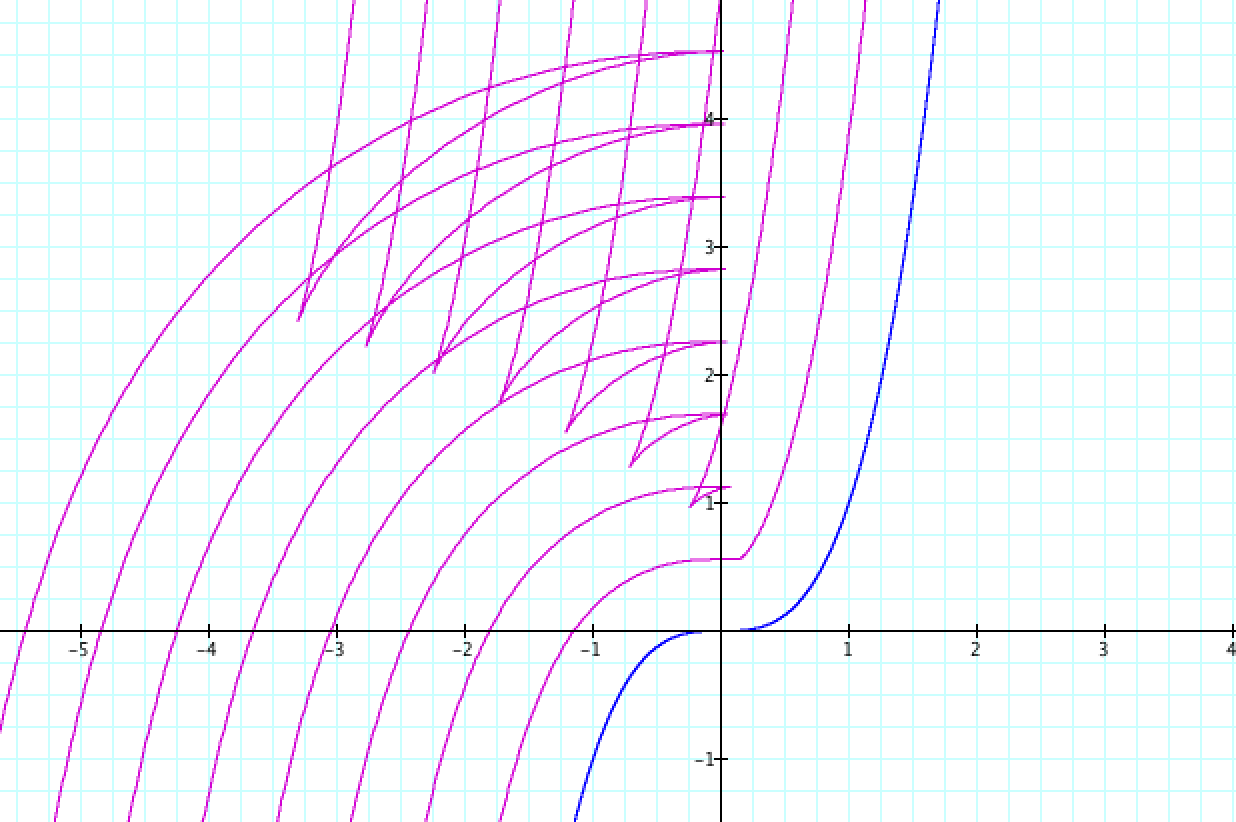
\includegraphics[width=\fw]{img/03-some-examples/06.png}
    \caption{$f(x) = x^3$, Divot Triangles}
    \vspace{4ex}
  \end{minipage} % end
  \begin{minipage}[b]{0.5\linewidth}
    \centering
    \label{example:7}
    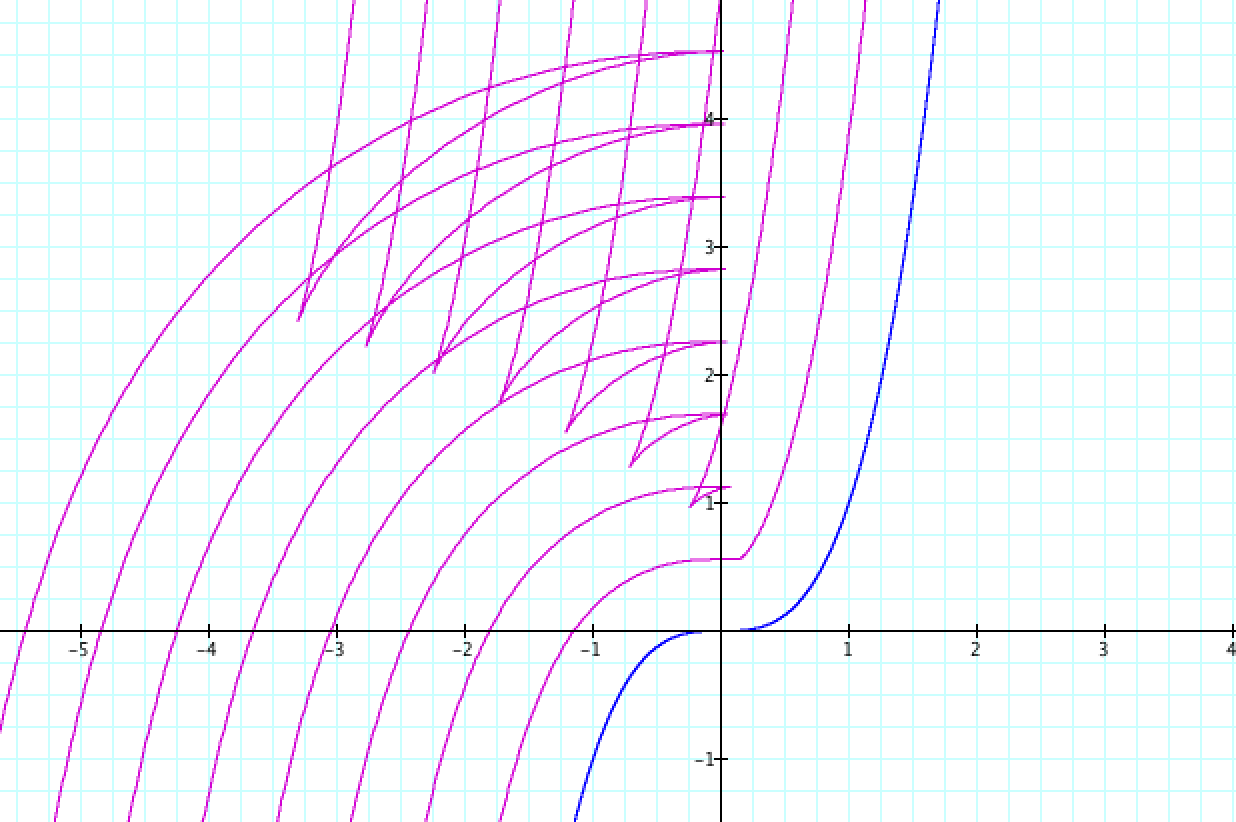
\includegraphics[width=\fw]{img/03-some-examples/07.png}
    \caption{$f(x) = x^3$, Divot Paths}
    \vspace{4ex}
  \end{minipage} % end
\end{figure}

\renewcommand\w{0.80\linewidth}

\begin{figure}[h!]
  \centering
  \begin{minipage}[b]{\w}
    \centering
    \label{example:8}
    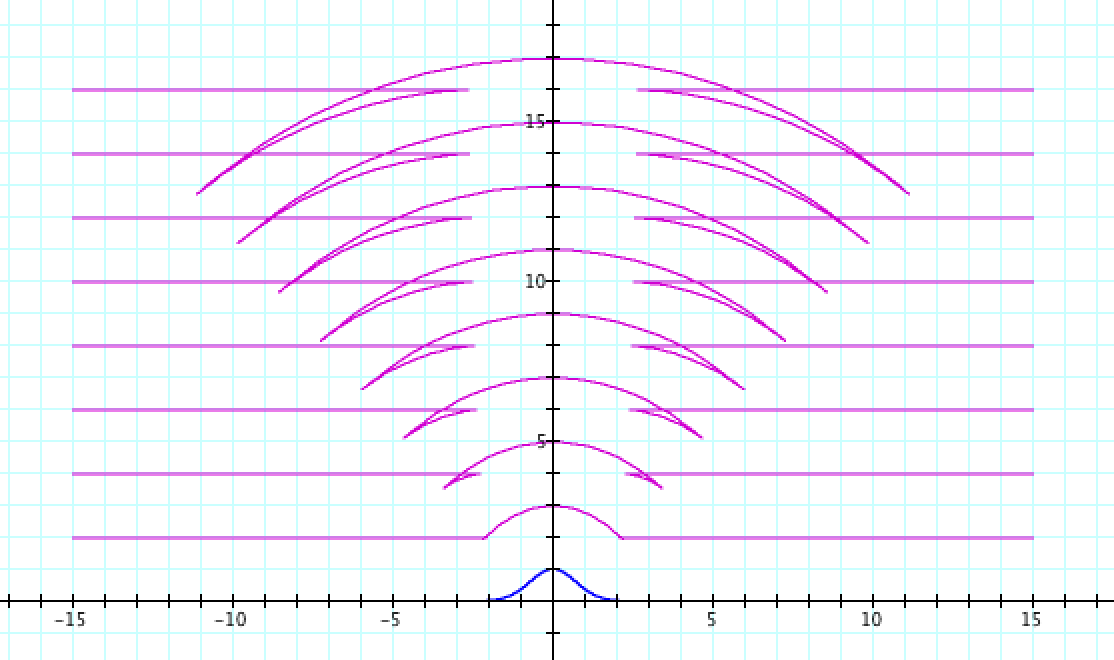
\includegraphics[width=\fw]{img/03-some-examples/08.png}
    \caption{$f(x) = e^{-x^2}$, Divot Paths}
    \vspace{4ex}
  \end{minipage} % end
\end{figure}

  \section{Statement of Intent}

This was as far as I made it working on the problem in high school. I’ve set out this college semester (Junior year) to utilize the more advanced mathematics tools I have since learned to combat my old nemesis and finally ``slay the dragon'', so to speak. My research on this topic has consisted of three main goals:

\begin{enumerate}
    \item Given an arbitrary continuously differentiable function $y = f(x)$, I want to be able to predict exactly where all of its crunch spots are in $\mathbb{R}^2$.
    \item If possible I want to find a closed formula for the actual $N$-Units Away Curves.
    \item For each crunch spots, I’d like to come up with a formula for (or at least some scientific understanding of) the three paths that the vertices of each divot triangle follow as N increases.
\end{enumerate}

At this point in the reading of this paper, I would definitely recommend that my readers pause here for a little while and play around with $N$-Units Away Curves themselves! They’re really fun. Simply go to Desmos.com and type in the following equations. Note that to make a derivative you type in ``d/dt''. Also make sure to set the t bounds to something like $-10 \leq t \leq 10$.

\renewcommand\w{0.8\linewidth}
\renewcommand\fw{0.9\linewidth}

\begin{figure}[H]
  \centering
  \begin{minipage}[b]{0.8\linewidth}
    \label{intent:1}
    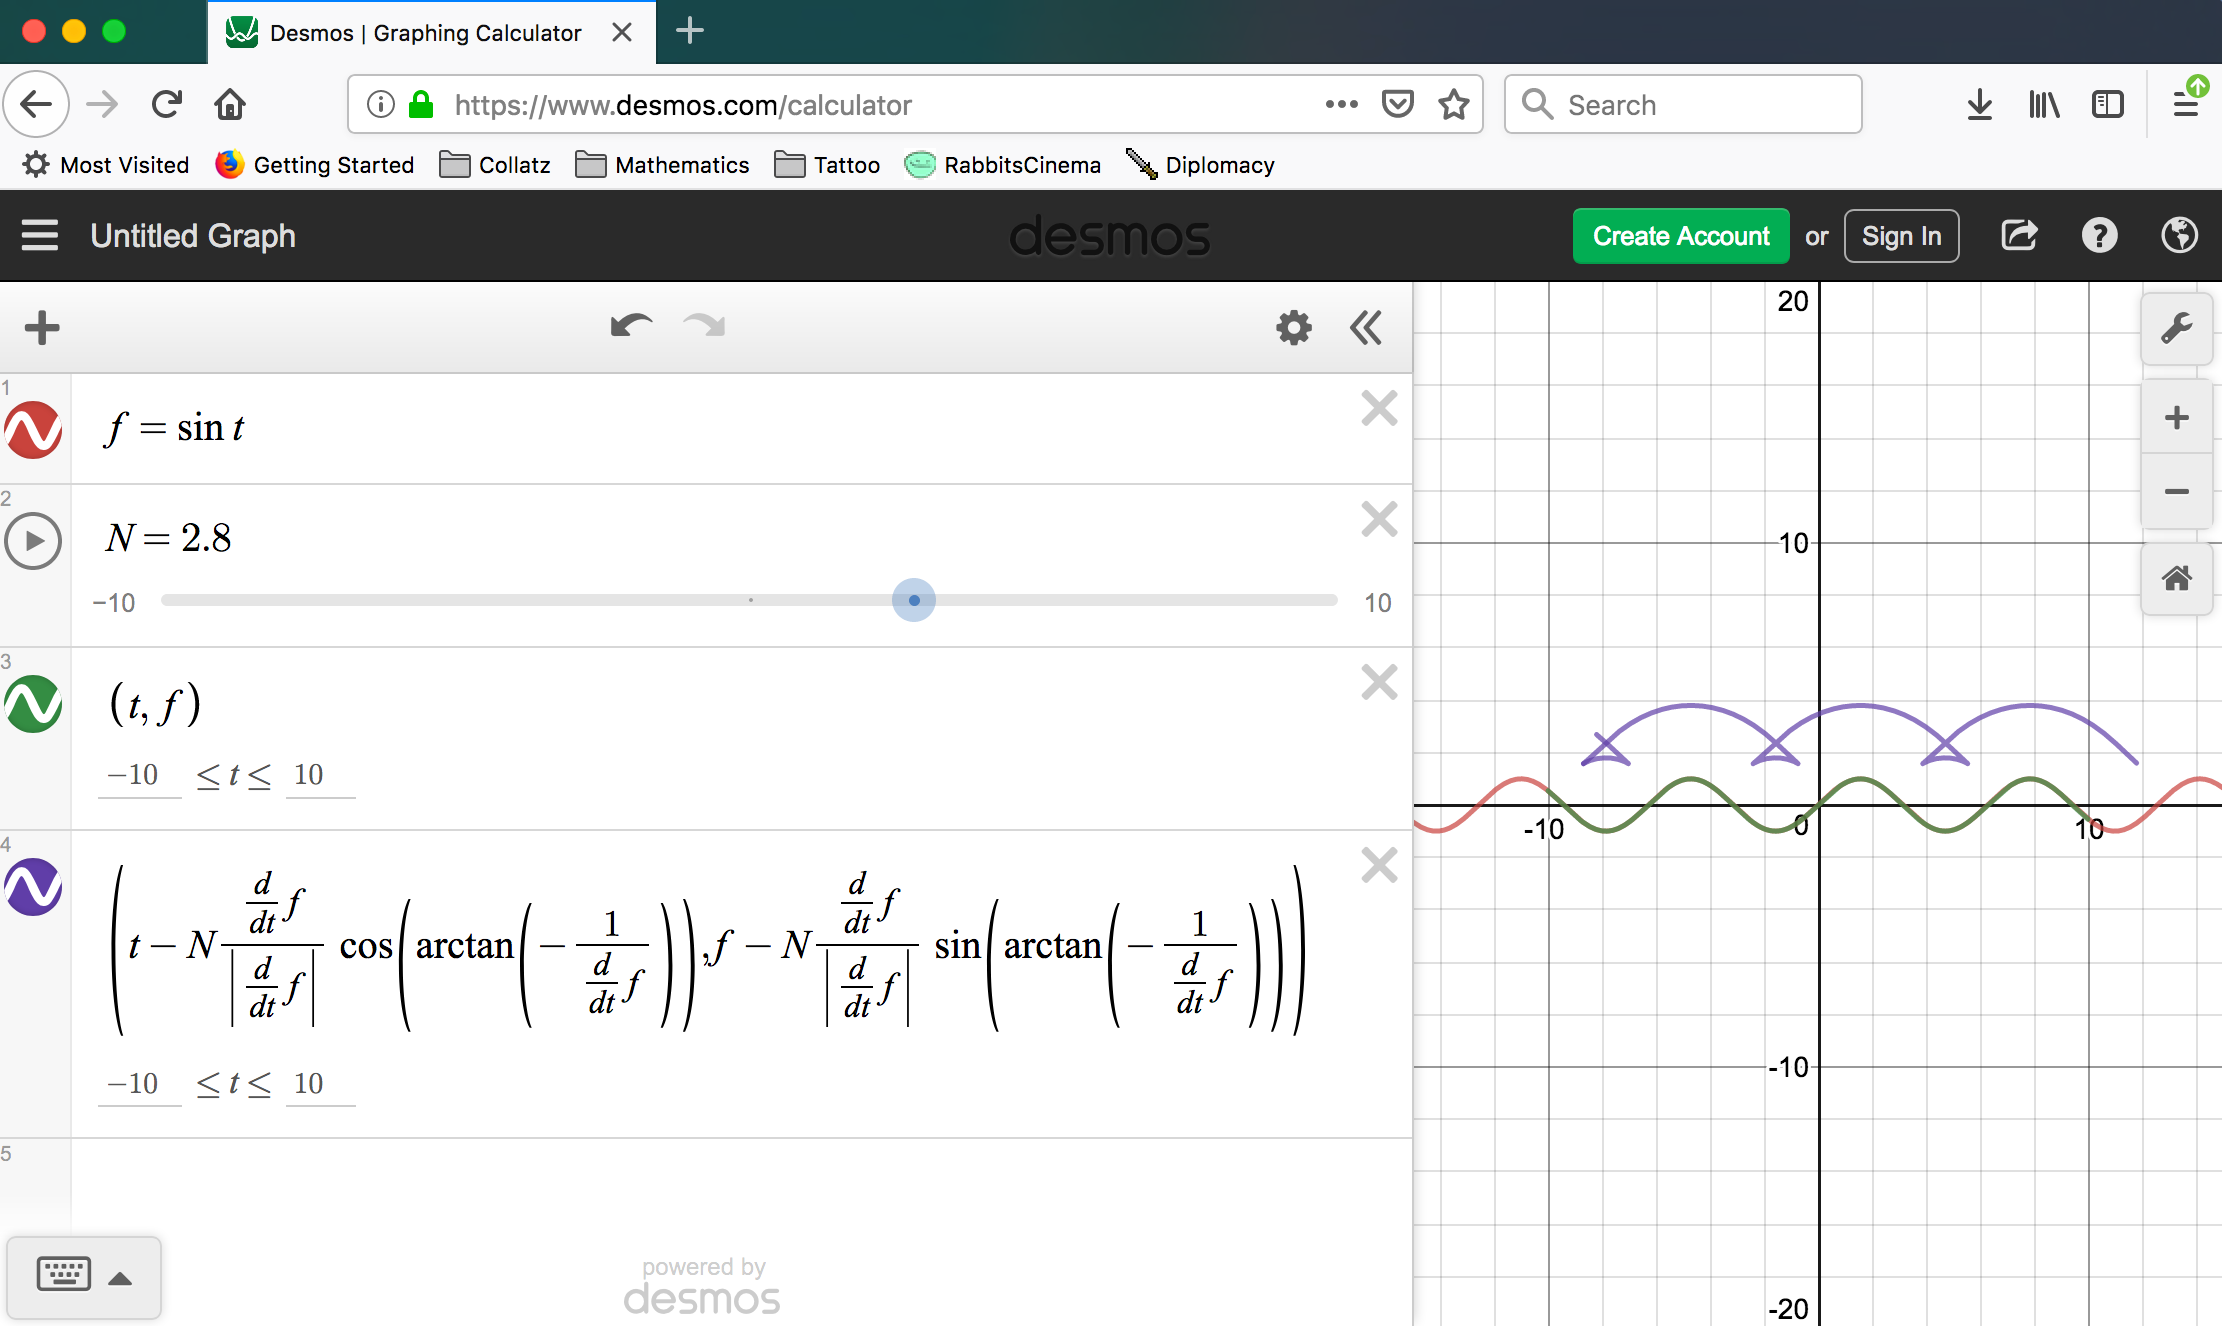
\includegraphics[width=\linewidth]{img/04-statement-of-intent/01.png}
    \caption{Desmos | Graphing Calculator}
  \end{minipage}
\end{figure}

... Then change Equation 1 to whatever function you’d like and drag the slidable $N$ value to
observe the behavior of the $N$-Units Away Curves. Have fun!

Now let’s get down to business...

  \newtheorem{definition}{Definition}

\section{Formal Definitions}

\begin{definition}
    Given a twice differentiable function $f(x)$ whose second derivative is continuous and some $N \in \mathbb{R}$, we define the \textbf{$N$-Units Away Curve} to be the collection of all points in $\mathbb{R}^2$ that are exactly $|N|$ units away from $y = f(x)$ along the normal line to $y = f(x)$ at some $x_o$. If $N$ is positive, include only those points that lie above the curve $y = f(x)$. If $N$ is negative, include only those points that lie below the curve.
\end{definition}

\begin{definition}
    \textbf{The ``Snipped'' $N$-Units Away Curve} is a function from $\mathbb{R}$ to $\mathbb{R}$ that we’ll denote $``f_N''(x)$ that can be created from the $N$-Units Away Curve by ``snipping'' off any of the divot triangles which occur every time the $N$-Units Away Curve crosses over itself. In the event that for a given value of $x$ multiple points on the N-Units Away Curve share that same $x$-value but have different y-values, we define $``f_N''(x)$ as taking on the $y$ value furthers from the original curve $y = f(x)$. Thus if $N$ is positive, it is the highest y value among them. If N is negative, it is the lowest.
\end{definition}

Examples:

\renewcommand\w{0.45\linewidth}
\renewcommand\fw{\linewidth}

\begin{figure}[H]
  \centering
  \begin{minipage}[b]{\w}
    \centering
    \label{formal:1}
    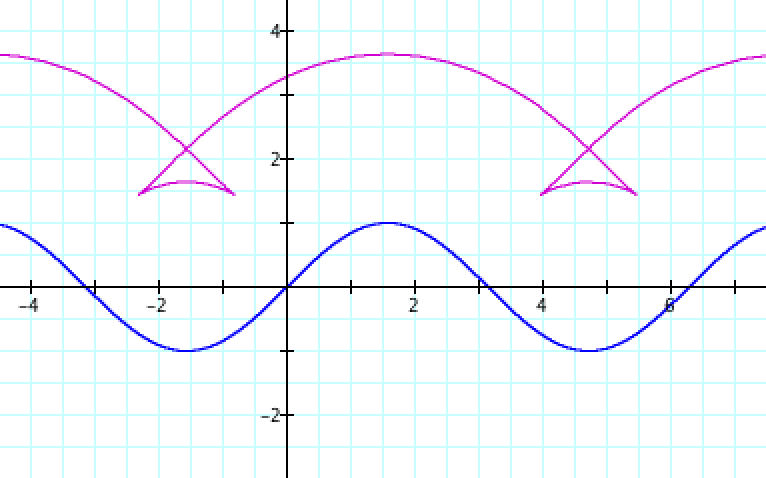
\includegraphics[width=\fw]{img/05-formal-definitions/01.png}
    \caption{$N$-Units Away Curve}
    \vspace{4ex}
  \end{minipage} % end
  \begin{minipage}[b]{\w}
    \centering
    \label{formal:2}
    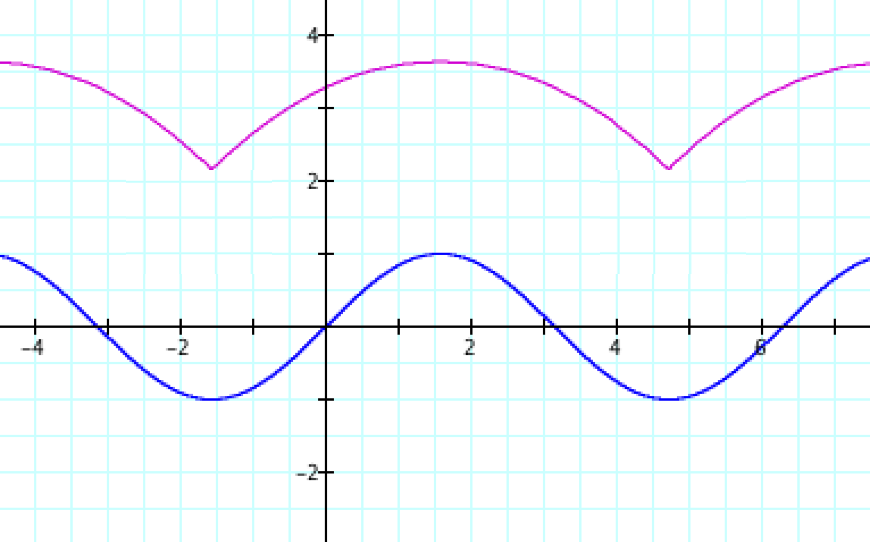
\includegraphics[width=\fw]{img/05-formal-definitions/02.png}
    \caption{``Snipped'' $N$-Units Away Curve}
    \vspace{4ex}
  \end{minipage} % end
\end{figure}

Just for the moment we'll take it as an assumption that $``f_N''(x)$ is defined on all of $\mathbb{R}$. We will return and establish this fact rigorously later on. Note that it was this ``snipped'' version of the $N$-Units Away Curve that my little kid self was drawing.

  \newtheorem{theorem}{Theorem}

\section{Existence and Uniqueness}

\begin{theorem}

  Given a twice differentiable function $f(x)$ whose second derivative is continuous and some $N \in \mathbb{R}$, $\exists$ exactly one unique $N$-Units Away Curve associated with that function.

\end{theorem}

\begin{proof}

  Consider the parametric formula for the $N$-Units Away Curve to $y = f(x)$: \firstFormula

  Since $f$ is both continuous and differentiable for $\forall t \in \mathbb{R}$, both $f(t)$ and $f'(t)$ necessarily exist as unique finite real values. Thus this gives that $\forall t, \exists$ exactly
  one unique associated point on the $N$-Units Away Curve. That same reasoning applied $\forall t \in (- \infty, \infty)$ gives us that the $N$-Units Away Curve exists and is unique.

\end{proof}

  \newcommand\bvec{\langle -f'(t), 1 \rangle}

\newcommand{\betterFormula}{

  \begin{equation} \tag{2}
    f_N(t) =
    \begin{bmatrix}
      x_N(t) \\
      y_N(t)
    \end{bmatrix} =
    \begin{bmatrix}
        t \\ f(t)
    \end{bmatrix} +
    \dfrac{N}{|\bvec|} \bvec
  \end{equation}

}

\renewcommand\bvec{\langle -f'(x_o), 1 \rangle}

\section{A Better Formula}

Next up, let’s establish rigorously a \textit{much} nicer parametric formula for the $N$-Units Away Curves. I figured this out after taking Multivariable Calc in college, and it’s a \textit{huge} improvement over my original high school formula.

Pick some $x_o \in \mathbb{R}$. There is exactly one point on the curve $y = f(x)$ corresponding to that location, namely $(x_o , f(x_o))$. A nice simple vector pointing in the direction of the tangent line to $y = f(x)$ at $x = x_o$ is $\langle 1, f'(x_o) \rangle$. Thus a nice simple vector
pointing in the direction of the normal line to $y = f(x)$ at $x = x_o$ is $\langle -f'(x_o), 1 \rangle$.

We want to establish a vector which points ``up'' along that normal line, but note that now unlike before we do not need to switch signs based on the sign of $f'(x_o)$! Also note that there is no longer any divide by zero issue encountered when $f'(x_o) = 0$. Nice! We want to have a unit normal vector: $\dfrac{\bvec}{|\bvec|}$ and then multiply this by N to get a vector that literally points from $(x_o, f(x_o))$ to a spot $N$ units away and in the ``up'' direction of the normal line to $y = f(x)$ at $x = x_o$. This gives us a \textit{vastly} new and improved version of the formula for $N$-Units Away Curves:

\betterFormula

  \section{Properties}

\begin{theorem}

  $N$-Units Away Curves have parametric continuity aka the curve has no gaps (even though it might well exhibit kinks or sharp bends.) Note: This, to me, is what lets us call them $N$-Units Away ``\textit{Curves}''.

\end{theorem}

% new vector with x_o
\newcommand\vo{
  % vector
  \newcommand\votemp{\langle -f'(x_o), 1 \rangle}
  \votemp \dfrac{ N }{ |\votemp| }
}

% new vector with x_n
\newcommand\vn{
  % vector
  \newcommand\vntemp{\langle -f'(x_n), 1 \rangle}
  \vntemp \dfrac{ N }{ |\vntemp| }
}

\begin{proof}

  Take some point $(x_o, f(x_o))$ on the curve $y = f(x)$. It’s associated point on the $N$-Units Away Curve is $
  \begin{bmatrix}
    x_o \\
    f(x_o)
  \end{bmatrix} + \vo$.

  Take some sequence of $\mathbb{R}$ values $(x_n)_{n \geq 1} \ni x_n \xrightarrow{} x_o$. Does the point on the $N$-Units away curve associated with $t = x_n, n = 1, 2, 3...$ approach that associated with $t = x_o$ as $n \xrightarrow{} \infty$? If it does, then by classical principles of Real Analysis we’ll know that the $N$-Units Away Curves have parametric continuity. Let’s see if that’s true.

  Consider $(x_n, f(x_n))$ as $n \xrightarrow{} \infty$. $x_n \xrightarrow{} x_o$. $f$ is twice differentiable and thus is also continuous, so we know that $f(x_n) \xrightarrow{} f(x_o)$. Thus $(x_n, f(x_n)) \xrightarrow{} (x_o, f(x_o))$.

  What of the vector $\vo$ as $n \xrightarrow{} \infty$? Since $f$ is twice differentiable that implies that $f'$ is continuous. Thus $f'(x_n) \xrightarrow{} f'(x_o)$. Putting this all together we arrive at as $n \xrightarrow{} \infty$, $
  \begin{bmatrix}
    x_n \\
    f(x_n)
  \end{bmatrix} + \vn
  \xrightarrow{}
  \begin{bmatrix}
    x_o \\
    f(x_o)
  \end{bmatrix} + \vo$.

  Thus the point on the $N$-Units Away Curve associated with $t = x_n$ approaches the point on the $N$-Units Away Curve for $t = x_o$ as $n \xrightarrow{} \infty$. The $N$-Units Away Curves are parametrically continuous.

\end{proof}

Before introducing the next three theorems, we’re going to take a moment and glance back at my little kid idea of drawing curves that stay the same distance away from each other. I mentioned on page 2 of this paper that ``as a child doodling, it seemed natural to then repeat the process and draw another curve that lay the same distance away from this new curve. I’d repeat the process a whole bunch of times.'' (figure $\ref{intro:4}$). There is a quiet assumption going on here though. My little kid self was actually making a second $N$-Units Away Curve \textit{from the original} $N$-Units Away Curve and then repeating that process. My adult mathematician self asks: can you make an $N$-Units Away Curve from an $N$-Units Away Curve? And if so, what is the result of the process? We shall build up to this over the course of the next three theorems.

\begin{theorem}

  $N$-Units Away Curves, as parametric curves, are differentiable.

\end{theorem}

% x_N'(t)
\newcommand{\xdern}{
  1 - N f''(t) ((-f'(t))^2 + 1)^{-1/2} + \dfrac{N}{2} f'(t) ( (-f'(t))^2 + 1) ^ {-3/2} (2 f'(t) f''(t))
}

% y_N'(t)
\newcommand{\ydern}{
  f'(t) - \dfrac{N}{2} f'(t) ((-f'(t))^2 + 1) ^ {-3/2} (2 f'(t) f''(t))
}

% new vector with t
\newcommand\vt{
  % vector
  \newcommand\vttemp{\langle -f'(t), 1 \rangle}
  \vttemp \dfrac{ N }{ |\vttemp| }
}


\begin{proof}

  \begin{equation*}
    f_N(t) =
    \begin{bmatrix}
      x_N(t) \\
      y_N(t)
    \end{bmatrix} =
    \begin{bmatrix}
      t \\
      f(t)
    \end{bmatrix} + \vt =
    \begin{bmatrix}
      t - N f'(t) ((-f'(t))^2 + 1)^{-1/2} \\
      f(t) + N f'(t) ((-f'(t))^2 + 1)^{-1/2}
    \end{bmatrix}
  \end{equation*}

  We can take this and derive each component:

  $x_N'(t) = \xdern$

  $y_N'(t) = \ydern$

  Note that these both always exist and are finite $\forall t \in (- \infty, \infty)$, thus giving us that the $N$-Units Away Curves are differentiable.

\end{proof}

\begin{theorem}

  For a given value of $t$, call it $t_o$, the $N$-Units Away Curve’s parametric derivative at $t$, aka $\dfrac{dy}{dx} = \dfrac{y_N'(t)}{x_N'(t)}$ is always equal to the derivative of the original curve at $t$, $f'(t)$. This is true regardless of the choice of $N$. Stated more precisely, $\forall t \land \forall N, y_N'(t) = f'(t) x_N'(t)$. (A conjecture first proposed by John Ennis.)

\end{theorem}

\begin{proof}

  $\forall t \land \forall N$,
  \begin{align*}
    LHS = & y_N'(t) = \ydern \\
    RHS = & x_N'(t) = \xdern
  \end{align*}

  Frankly? Yuck. Why in the world would these two massive equations always equal each other? Let’s proceed forward slowly and thoughtfully and establish that they are, in fact, equivalent. As $((-f'(t))^2 + 1) ^ {-3/2}$ can never achieve a value of 0, we can safely multiply both sides by it to obtain:
  \begin{align*}
    LHS = & f'(t) ((-f'(t))^2 + 1) ^ {-3/2} - N f'(t) f''(t) \\
    RHS = & x_N'(t) = f'(t) ((-f'(t))^2 + 1) ^ {-3/2} - N f'(t) f''(t) ((f'(t) ^ 2 + 1) + N (f'(t))^3 f''(t)
  \end{align*}

  And subtract $((-f'(t))^2 + 1) ^ {-3/2}$ from both sides. In the case that $N = 0$, then \textit{of course} the derivative of the $N$-Units Away Curve is the same as that of the original function. The $0$-Units Away Curve is the original function! In the case that $N \neq 0$, we can divide both sides by -$N$, giving us:
  \begin{align*}
    LHS = & f'(t)f''(t) \\
    RHS = & f'(t)f''(t) ((f'(t))^2 + 1) - ((f'(t))^3 f''(t) = f'(t)f''(t)
  \end{align*}, confirming the theorem.

\end{proof}

\begin{theorem}

  The $N_2$-Units Away Curve of the $N_1$-Units Away Curve of $y = f(x)$ is precisely the $(N_1 + N_2)$-Units Away Curve of $y = f(x)$.

\end{theorem}

\begin{proof}

  The fact that all the $N$-Units Away Curves share the same derivative for the same value of t implies that they all share the same normal line. The only case where this might not be true is very specifically when $x_N'(t) = 0$. But then by $y_N'(t) = f'(t) x_N'(t)$ we have that $y_N'(t)$ is also 0. But that means that the $N$-Units Away Curve is not even ``drawing more line'' at that t value. The $N$-Units Away Curve has briefly stopped. The instant that it resumes motion, it will once again be cut at $90 ^{\circ}$ by the normal line.

  Thus since the normal line to the original curve at $x = x_o$ cuts through all of the $N$-Units Away Curves precisely at a $90^{\circ}$ angle, we can see that moving $N_1$ units along this normal line and then moving $N_2$ units further along this same line is equivalent to moving $(N_1 + N_2)$ units along the normal line from the original curve. Thus the $N_2$-Units Away Curve \textit{of} the $N_1$-Units Away Curve of $y = f(x)$ is precisely the $(N_1 + N_2)$-Units Away Curve of $y = f(x)$.

\end{proof}

Ok... Now on to the main topics of this paper.

  \newcommand\fh{}

\newcommand\figuresI{

  \renewcommand\w{0.3\linewidth}
  \renewcommand\fw{0.7\textwidth}
  \renewcommand\fh{0.3\textheight}

  \begin{figure}[H]
    \begin{minipage}[b]{\w}
      \centering
      \label{crunch:2}
      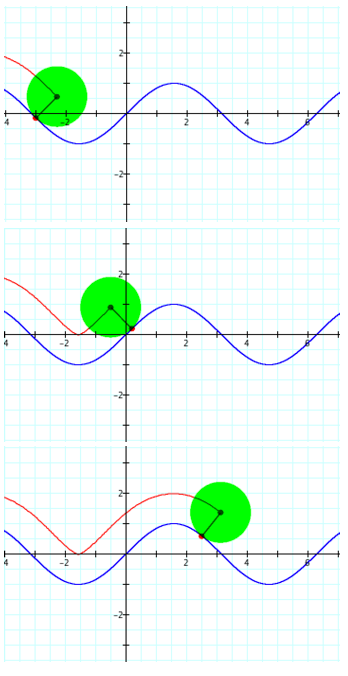
\includegraphics[width=\fw, height=\fh, keepaspectratio]{img/09-crunch/02.png}
      \caption{Caption}
      \vspace{4ex}
    \end{minipage} % end
    \begin{minipage}[b]{\w}
      \centering
      \label{crunch:3}
      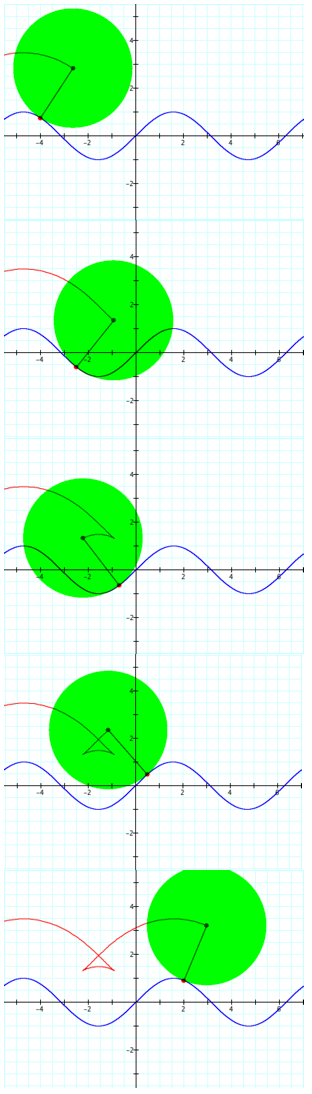
\includegraphics[width=\fw, height=\fh, keepaspectratio]{img/09-crunch/03.png}
      \caption{Caption}
      \vspace{4ex}
    \end{minipage} % end
    \begin{minipage}[b]{0.5\linewidth}
      \centering
      \label{crunch:4}
      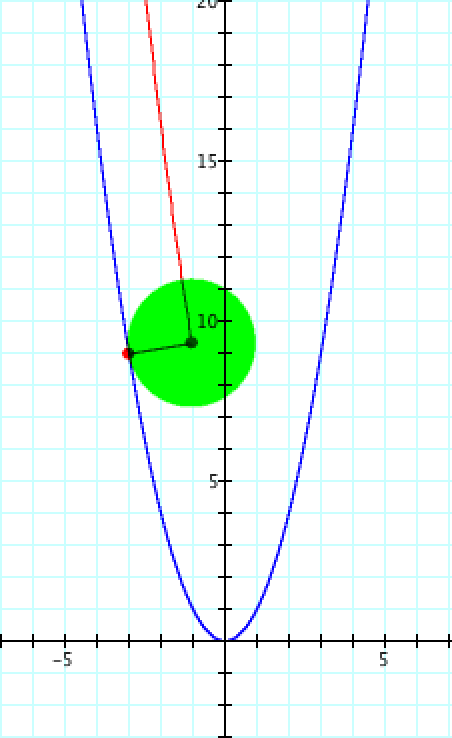
\includegraphics[width=\fw, height=\fh, keepaspectratio]{img/09-crunch/04.png}
      \caption{Caption}
      \vspace{4ex}
    \end{minipage} % end
  \end{figure}

}

\newcommand\figuresII{

  \renewcommand\w{0.4\linewidth}
  \renewcommand\fw{0.9\textwidth}
  \renewcommand\fh{0.3\textheight}

  \begin{figure}[H]
    \centering
    \begin{minipage}[b]{\w}
      \centering
      \label{crunch:5}
      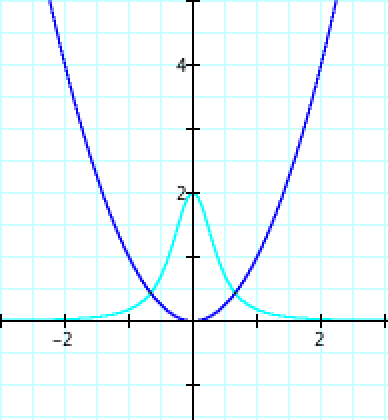
\includegraphics[width=\fw, height=\fh, keepaspectratio]{img/09-crunch/05.png}
      \caption{Caption}
      \vspace{4ex}
    \end{minipage} % end
    \begin{minipage}[b]{0.5\linewidth}
      \centering
      \label{crunch:6}
      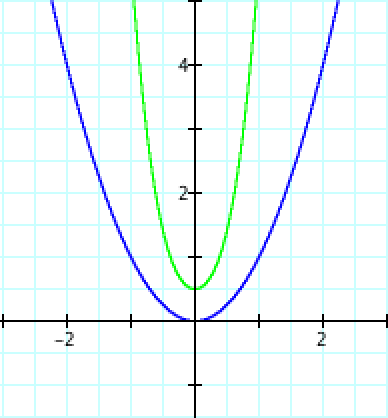
\includegraphics[width=\fw, height=\fh, keepaspectratio]{img/09-crunch/06.png}
      \caption{Caption}
      \vspace{4ex}
    \end{minipage} % end
  \end{figure}

}

\newcommand\figuresIII{

  \renewcommand\w{0.9\linewidth}
  \renewcommand\fw{0.9\textwidth}
  \renewcommand\fh{0.2\textheight}

  \begin{figure}[H]
    \centering
    \begin{minipage}[b]{\w}
      \centering
      \label{crunch:7}
      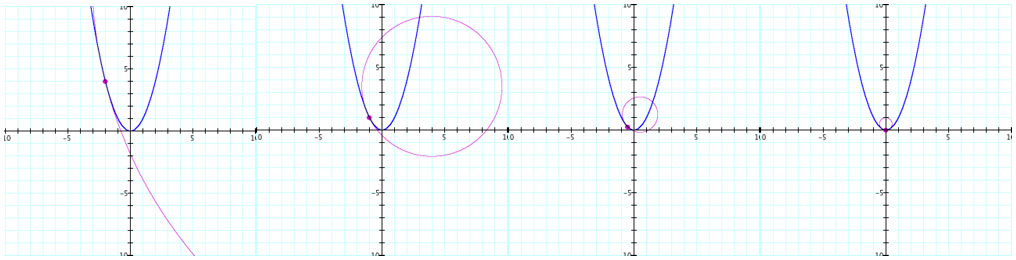
\includegraphics[width=\fw, height=\fh, keepaspectratio]{img/09-crunch/07.png}
      \caption{Caption}
      \vspace{4ex}
    \end{minipage} % end
    \begin{minipage}[b]{\w}
      \centering
      \label{crunch:8}
      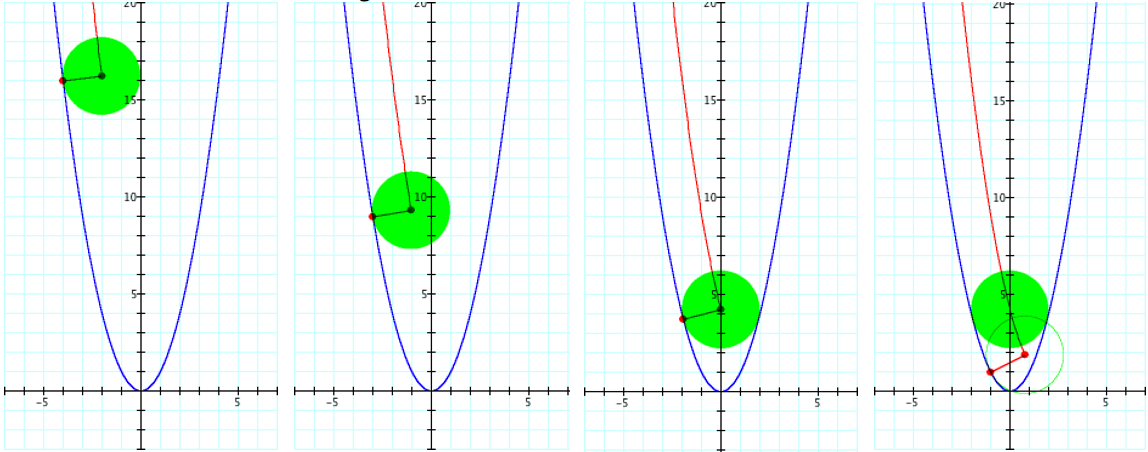
\includegraphics[width=\fw, height=\fh, keepaspectratio]{img/09-crunch/08.png}
      \caption{Caption}
      \vspace{4ex}
    \end{minipage} % end
  \end{figure}

}

\newcommand\figuresIV {

  \renewcommand\w{0.2\linewidth}
  \renewcommand\fw{0.9\textwidth}

  \begin{figure}[H]
    \centering
    \begin{minipage}[b]{\w}
      \centering
      \label{crunch:9}
      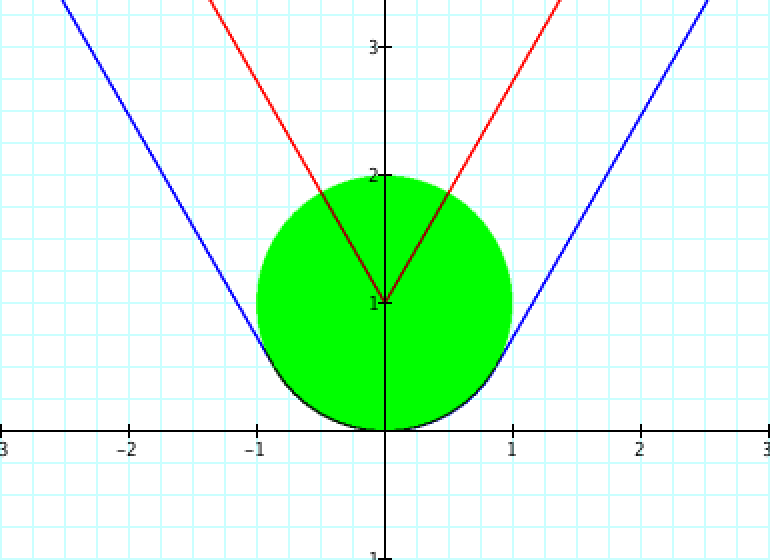
\includegraphics[width=\fw]{img/09-crunch/09.png}
      \caption{Caption}
    \end{minipage}
    \begin{minipage}[b]{\w}
      \centering
      \label{crunch:10}
      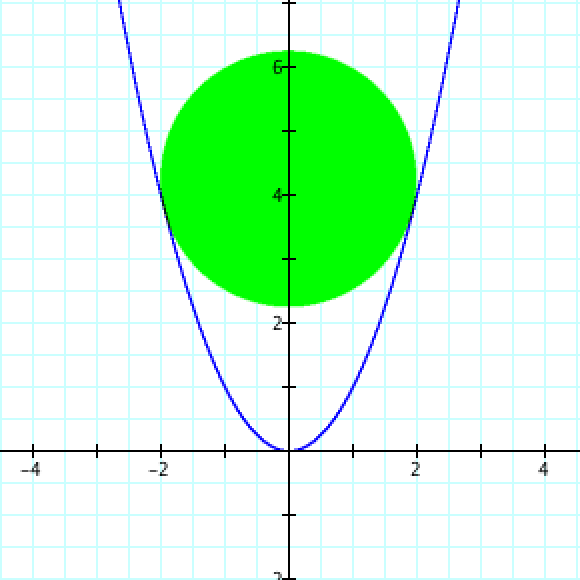
\includegraphics[width=\fw]{img/09-crunch/10.png}
      \caption{Caption}
    \end{minipage}
    \begin{minipage}[b]{\w}
      \centering
      \label{crunch:11}
      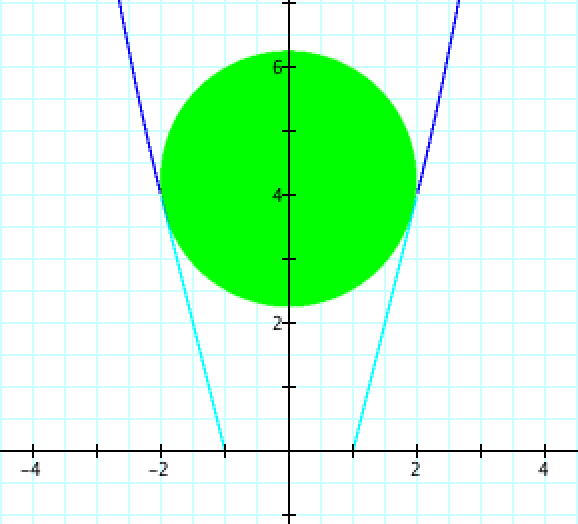
\includegraphics[width=\fw]{img/09-crunch/11.png}
      \caption{Caption}
    \end{minipage}
    \begin{minipage}[b]{\w}
      \centering
      \label{crunch:12}
      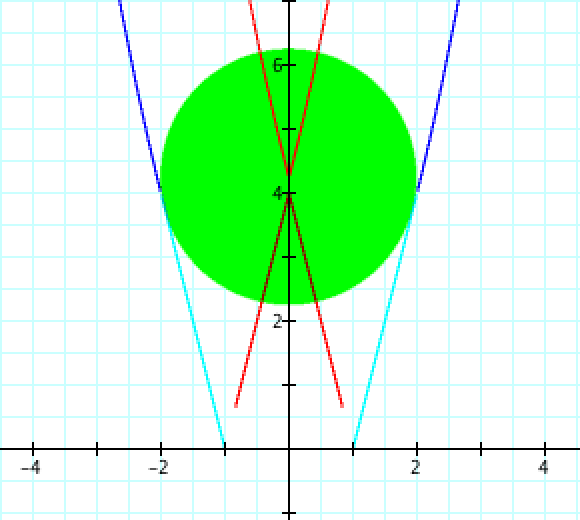
\includegraphics[width=\fw]{img/09-crunch/12.png}
      \caption{Caption}
    \end{minipage}
  \end{figure}

}

\newcommand\figuresV{

  \renewcommand\w{0.40\linewidth}
  \renewcommand\fw{0.90\textwidth}

  \begin{figure}[h]
    \centering
    \begin{minipage}[b]{\w}
      \centering
      \label{crunch:13}
      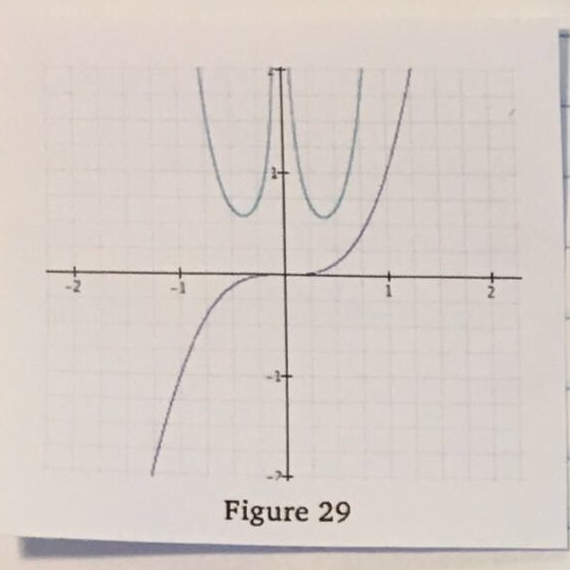
\includegraphics[width=\fw]{img/09-crunch/13.png}
      \caption{Caption}
    \end{minipage}
    \begin{minipage}[b]{\w}
      \centering
      \label{crunch:14}
      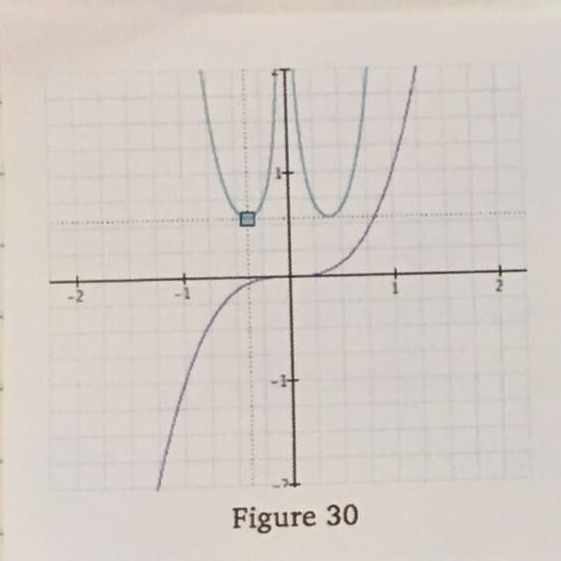
\includegraphics[width=\fw]{img/09-crunch/14.png}
      \caption{Caption}
    \end{minipage}
    \begin{minipage}[b]{\w}
      \centering
      \label{crunch:15}
      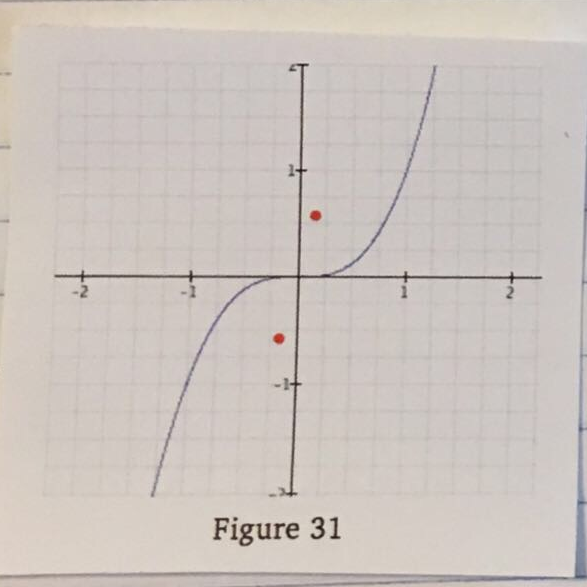
\includegraphics[width=\fw]{img/09-crunch/15.png}
      \caption{Caption}
    \end{minipage}
    \begin{minipage}[b]{\w}
      \centering
      \label{crunch:16}
      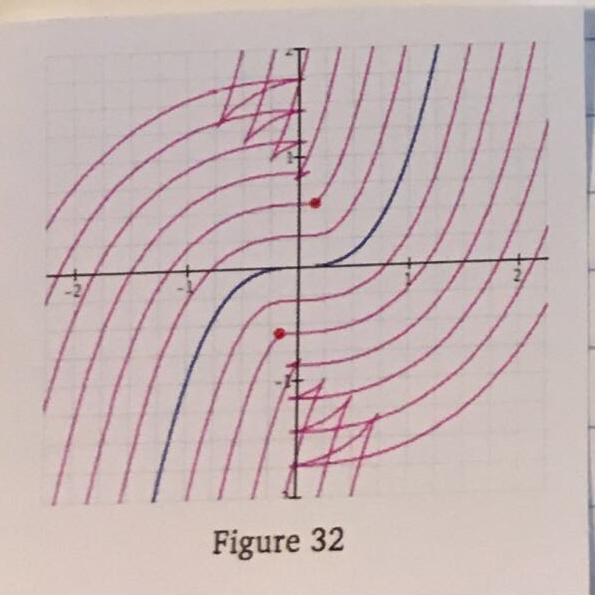
\includegraphics[width=\fw]{img/09-crunch/16.png}
      \caption{Caption}
    \end{minipage}
  \end{figure}

}

\section{Finding Crunch Spots}

\renewcommand\w{0.25\linewidth}
\renewcommand\fw{0.9\linewidth}

\begin{wrapfigure}{l}{\w}
  \label{crunch:1}
  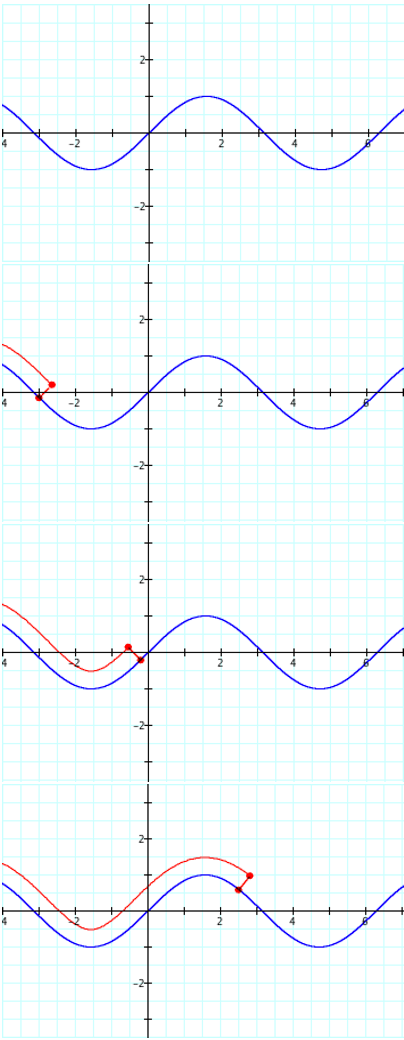
\includegraphics[width=\fw]{img/09-crunch/01.png}
  \caption{Caption}
\end{wrapfigure}

Let’s do a math thought experiment! We’re going to build a little imaginary railroad track. Imagine now that you’re standing in the Nevada desert and you wish to lay down a railroad track. Take your favorite continuously differentiable function $f(x)$. Pick a spot on the dirt to be the origin. Let the $x$-axis be East-to-West and let the $y$-axis be North-to-South. Now plot your function $f(x)$ across the desert sands using metal to form one of the railroad track rails. For the sake of conversation let’s call it the right rail. Place a little sliding metal bit onto the track that we can push back and forth along the rail. Connect to it a metal bar of some set fixed length N that will at all times be perpendicular to the rail. Fix to the end of the metal bar a jumbo sized red magic marker that will draw upon the sand as the sliding metal bit moves along $f(x)$. As the sliding metal bit is pushed along f(x), the bar and marker will draw the left rail, aka the $N$-Units Away Curve. This set up is diagrammed in figure $\ref{crunch:1}$. In this diagram we used $f(x) = sin(x)$.

Now add one more element to the scenario. Place onto the end of the metal beam a cool little LED light that will project a green circle of radius $N$ onto the desert sand. It ``rolls along'' the original function a little like a marble. This is diagrammed in figures $\ref{crunch:2}$ and $\ref{crunch:3}$. We see that this green marble rolls smoothly along the $y = f(x)$ function with its center moving precisely along the $N$-Units Away Curve. We see that for small values of $N$ (fig $\ref{crunch:4}$), the green marble does not intersect the original function $y = f(x)$ at all. We see that it does intersect the original function for higher $N$ values (fig $\ref{crunch:3}$).

Now let us leave behind the Nevada desert and simply roll marbles down some functions! Let’s take the example of $y = x^2$. Take a fairly sizable marble, perhaps one of radius 2 and roll it down the curve! The following occurs:

We see that the marble gets stuck at the bottom of the parabola and cannot continue following the path of the $N$-Units Away Curve. The curve of the function got ``too tight'' for the marble to fit into. Thus we see there is correlation between the crunch spots of the $N$-Units Away Curves and portions of the original function that have maximum curvature. How can we express this connection with mathematical rigor? Luckily for us, there is already a concept of ``curvature'' in Calculus.

To quote the classic James Stewart \textit{Calculus} textbook, ``the curvature of a function at a given point is a measure of how quickly the curve changes direction at that point'' (863.) If a tiny car were to drive along the path of the function, the curvature at a given value of $x$ gives a measure of how significantly the steering wheel of the tiny car is turned. It has formula $\kappa (x) = \dfrac{|f''(x)|}{[1 + (f'(x))^2]^{3/2}}$.

\figuresI

Let’s plot the graph of a function and its curvature. (Fig $\ref{crunch:5}$) The function will be dark blue and the curvature turquoise. If you take the multiplicative inverse of the curvature, $\dfrac{1}{\kappa (x)}$, you obtain a concept from differential geometry called the ``radius of curvature.'' We denote it by $R(x)$. It’s another way to measure how quickly the function is turning. It is equal to the radius of the circular arc which best approximates the curve at that point. (Fig $\ref{crunch:6}$) displays $y = x^2$ next to the graph of its radius of curvature, shown in green. For an example of radius of curvature in action, here is a look at a series of points on $y = x^2$ and their ``best approximating circles'' (Fig $\ref{crunch:7}$).

Let’s go on another little thought experiment. Suppose you want to roll a marble of positive radius $N$ along the function $y = f(x)$. You’re going to roll it smoothly along the curve, making sure it contacts the function at every $x$ value. What does it mean mathematically to find a spot where the marble gets ``stuck'' as in the rightmost image of (Fig $\ref{crunch:8}$)?

\figuresII

We observe now that the path that the marble’s centerpoint follows is precisely the Snipped $N$-Units Away Curve. The reasoning for this is the following: If the marble has simply rolled along pleasantly and nothing out of the usual has occurred, then the location of its centerpoint will perfectly coincide with the $N$-Units Away Curve point created by moving $N$ units away from the function along the normal to where the ball is touching. The strange exotic behavior only happens when the ball is obstructed in its path, aka it gets ``stuck'' The marble only gets stuck when it additionally contacts a second portion of the curve. In this event we know that there exist two distant values of $t$ which result in the same point on the $N$-Units Away Curve. Call them $t_1$ and $t_2$. Let $x_1$ and $x_2$ be the $x$-values of the original function at $t_1$ and $t_2$. What are the possible scenarios of what function $y = f(x)$ could be doing on open interval $(x_1, x_2)$?

\figuresIII

Case 1, some value $x_o \in (x_1, x_2)$ gives a point $(x_o, f(x_o))$ which occurs inside the green area of the marble. This is a contradiction, as the marble cannot have rolled so far that part of the function it was rolling on is now jammed inside of it. It surely would have gotten stuck the moment it first made contact with two points of the function.

Case 2, every value $x_o \in (x_1, x_2)$ is such that $(x_o, f(x_o))$ lies exactly on the bottom edge of the circle. This means that on that interval the function is precisely a circular arc with the same radius as the marble. Immediately before and after interval $(x_1, x_2)$ the marble will have no trouble rolling along the function. During interval $(x_1, x_2)$ it will rest snuggly in that little circular arc immobile. We see that no divot triangle or strange exotic behavior occurs. Note that this is a region whereon the radius of curvature is precisely $N$. This scenario is diagrammed in Figure $\ref{crunch:9}$ with specially constructed branching function:

\begin{equation*}
  y =
  \begin{cases}
  % case 1
    % expression
    \sqrt{3} \left( x - \dfrac{\sqrt{3}}{2} \right) + \dfrac{1}{2}, &
    % condition
    x \in \left( -\infty, - \dfrac{\sqrt{3}}{2} \right]
    \\
  % case 2
    % expression
    - \sqrt{1 - x^2} + 1, &
    % condition
    x \in \left( - \dfrac{\sqrt{3}}{2}, \dfrac{\sqrt{3}}{2} \right)
    \\
  % case 3
    % expression
    - \sqrt{3} \left( x + \dfrac{\sqrt{3}}{2} \right) + \dfrac{1}{2}, &
    % condition
    x \in \left[ \dfrac{\sqrt{3}}{2}, \infty \right)
  \end{cases}
\end{equation*}

Case 3, at least some value $x_o \in (x_1, x_2)$ gives a point $(x_o, f(x_o))$ which occurs below the marble and does make contact with it (Fig $\ref{crunch:10}$). For any point of the function to be below the marble, it means that the function had to both depart away from the marble and then return back to it at some $x_3 < x_4$ both $\in [x_1, x_2]$. Consider the tangent lines to the function $y = f(x)$ at $x_3 \land x_4$ (Fig $\ref{crunch:11}$). They travel \textit{closer} to one another, thus meaning that the function $y = f(x)$ must at some point on $(x_3, x_4)$ take an even sharper turn than the bottom circular edge of the marble. This guarantees that somewhere on $(x_1, x_2)$ the function’s radius of curvature is less than $N$.

\figuresIV

Extending those tangent lines shows that immediately after $x_3$ the left tangent line (which $f(x)$ approximates, even if only briefly) spawns an $N$-Units Away point which is to the \textit{right} of the center point of the marble (Fig $\ref{crunch:12}$). Likewise just before $x_4$ the right tangent line (which $f(x)$ approximates) spawns an $N$-Units Away point which is to the left of the center point of the marble. Both of these points are also \textit{below} the centerpoint thus guaranteeing that the N-Units Away Curve will now fail the Vertical Line Test and we are seeing a budding divot triangle, occurring \textit{below} the Snipped N-Units Away Curve.

When you are rolling a marble of radius $N$ towards an interval of the function with radius of curvature less than $N$, we will always find a divot triangle.

But it works the other way around too. If you ever find a divot triangle on an $N$-Units Away Curve, then precisely at the apex of the triangle a marble of radius $N$ would have gotten stuck. The light blue tangent lines continue towards one another getting \textit{closer}, thus necessarily meaning that the function $y = f(x)$ took a sharper turn than the bottom circular edge of the marble. Like before, this guarantees that somewhere on $(x_3, x_4)$ the function had radius of curvature less than $N$.

Thus, $f(x)$ achieves a radius of curvature $ < N \iff $ a divot triangle is present.

This lets us precisely locate where all of the divot triangles first appear! The $N$-Units Away Curve for $y = f(x)$ will ``crunch'' upon itself and spawn a divot triangle at exactly those values of $x$ which gives local minimums of the radius of curvature of $f(x)$. Furthermore the critical value of $N$ which causes the crunching phenomenon to occur will be precisely the value of that local minimum of the radius of curvature.

All of the above was thought out with the assumption that $N$ is positive. If $N$ is negative, you have a marble rolling along the ``ceiling'' curve of a function with reversed gravity pointing upwards. Marbles can only get stuck when the function curves \textit{towards} them. Thus crunch spots above the function will be created when the function is concave up aka when $f''$ is positive and crunch spots below the function will be created when the function is concave down aka when $f''$ is negative.

We now summarize all of these findings into one big theorem:

\begin{theorem}

  A twice differentiable function $f(x)$ whose second derivative is continuous produces a unique crunch spot of its $N$-Units Away Curves at precisely the values of $x$ which give the radius of curvature function $R(x)$ a local minimum. The crunch spot of $\mathbb{R}^2$ associated with each minimum $x_m$ is found exactly $R(x_m)$ units along the normal line to the function $y = f(x)$ at $x = x_m$ in the direction up or down corresponding to the sign of $f''$. . This location can be found by plugging $t_m = x_m$ into the equation for the $\left( \dfrac{f''(t_n)}{|f''(t_n)|} R(t_n) \right)$-Units Away Curve.

\end{theorem}

\subsection{An example}

Let us now do an example to show the true power of this theorem.

\figuresV

Take as our function a classic: $y = x^3$. Where are its crunch spots to be located? Plot the function $y = x^3$ and now also plot its radius of curvature function: $R(x) = \dfrac{(1 + f'(x))^2)^{3/2}}{|f''(x)|}$. Figure $\ref{crunch:13}$ displays both of these. Using computerized approximation, we see that $R(x)$ has two local minimums, one at $(-0.386, 0.567)$ the other at $(0.386, 0.567)$... (Fig $\ref{crunch:14}$).

The previous theorem tells us that we should be able to find the first of the two crunch spots on $\mathbb{R}^2$ by plugging $t_{m_1} = -0.386$ and $ N = \dfrac{f''(t_{m_1})}{|f''(t_{m_1})|} 0.567 = -0.567 $ into Formula 2 for the $N$-Units Away Curve: $ f_N(t) =
\begin{bmatrix}
  t - N f'(t) ((f'(t))^2 + 1)^{-1/2} \\
  f(t) + N ((f'(t))^2 + 1)^{-1/2}
\end{bmatrix} $.

\newcommand\N{}
\newcommand\temp{}

\begin{center}
  \renewcommand\N{-0.567}
  \renewcommand\temp{-0.366}
  $
  \implies
  f_{\N}(\temp) =
  \begin{bmatrix}
    \temp - (\N) f'(\temp) ((f'(\temp))^2 + 1)^{-1/2} \\
    f(\temp) + (\N) ((f'(\temp))^2 + 1)^{-1/2}
  \end{bmatrix} =
  \begin{bmatrix}
    -0.155 \\
    -0.575
  \end{bmatrix}
  $
\end{center}

Doing the same with $t_{m_2} = 0.366$ and N = $\dfrac{f''(t_{m_2})}{|f''(t_{m_2})|} 0.567 = 0.567$ gives:

\begin{center}
  \renewcommand\N{0.567}
  \renewcommand\temp{0.366}
  $
  \implies
  f_{\N}(\temp) =
  \begin{bmatrix}
    \temp - \N f'(\temp) ((f'(\temp))^2 + 1)^{-1/2} \\
    f(\temp) + \N ((f'(\temp))^2 + 1)^{-1/2}
  \end{bmatrix} =
  \begin{bmatrix}
    0.155 \\
    0.575
  \end{bmatrix}
  $
\end{center}

These two points are plotted net to $y = x^3$ in figure $\ref{crunch:15}$. Are these the crunch spots?

Figure $\ref{crunch:16}$ shows that indeed these two points are none other than exactly the two crunch spots for $y = x^3$.

  \section{A Constructed Formula for the Snipped N-Units Away Curve}

When we first defined the Snipped $N$-Units Away Curve in section 5, we took it as an assumption that it was a function $``f_N''(x)$ on $x$ from $\mathbb{R} \xrightarrow{} \mathbb{R}$. How do we know it is necessarily defined on all of $\mathbb{R}$? $\forall$ values of $x$ there is an associated point on the regular $N$-Unis Away Curve which we know never has an $x$-value location outside of $(x - N, x + N)$. Take some arbitrary extremely negative $x$-value $x_L$ and an arbitrary extremely positive $x$-value $x_R$. We know $\exists$ two points on the $N$-Units Away Curve that are on $(x_L - N, x_L + N)$ and $(x_R - N, x_R + N)$ respectively. As the $N$-Units Away Curve has parametric continuity, we know it has no gaps. It necessarily crosses all $x$ values between $x_L + N$ and $x_R - N$, and we  may place those as far off towards the two infinities as we would like. The Snipped $N$-Units Away Curve is necessarily defined on all of $\mathbb{R}$.

How can we possibly learn more about this function $``f_N''(x)$? Well, we know from the previous section that the Snipped $N$-Units Away Curve is precisely the point that a marble of radius $N$'s centerpoint would follow were it to roll along the function (assume for a positive $N$).

\renewcommand\w{0.35\linewidth}
\renewcommand\fw{0.9\linewidth}

\begin{wrapfigure}{l}{\w}
  \label{constructed:1}
  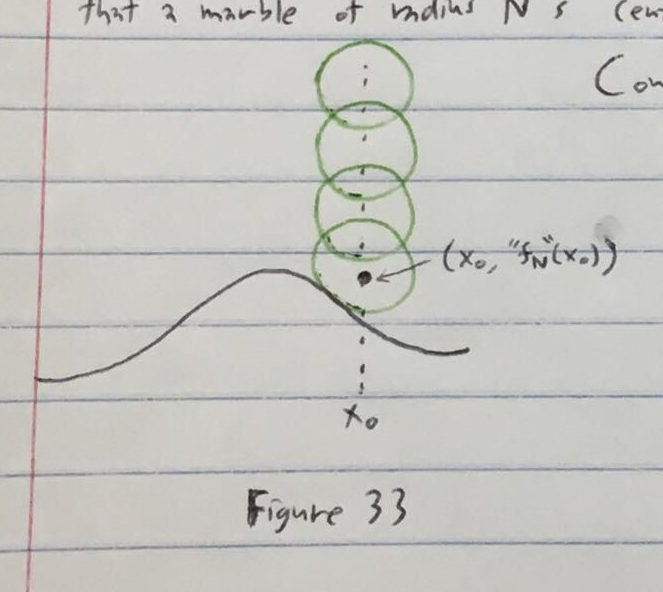
\includegraphics[width=\fw]{img/10-constructed/01.png}
  \caption{Caption}
\end{wrapfigure}

Consider the following... Choose your favorite value $x = x_o$. Take a marble of radius $N$ and gradually lower it down towards the function. The moment it first contacts the function $y = f(x)$, stop right there. This is exactly the location that the marble would assume were it rolling along the function at $x = x_o$. The $y$-value of the centerpoint right there is thus equal to $``f_N'(x_o)$.

Let's rewind a bit and think through this more mathematically. Take your function $y = f(x)$ and suspend a marble of radius $N$ way up above the curve directly above $\exists x = x_o$. This circle has equation $(y - y_c)^2 + (x - x_o)^2 = N^2$, where $y_c$ us the moveable height of the centerpoint of the marble. Solving for $y$, we get that the bottom half of the semi-circle of the marble can be described by $y = - \sqrt{ N^2 -(x - x_o)^2 } + y_c$. What we seek is the very highest $y_c$ value $\ni$ the function and this bottom half of the marble touch, aka what is the highest possible $y_c \ni (- \sqrt{ N^2 - (x - x_o)^2 } + y_c) - f(x)$ has a zero on interval $x \in (x_o - N, x_o + N)$?

\renewcommand\fw{0.8\linewidth}

\begin{figure}[h]
  \centering
  \label{constructed:2}
  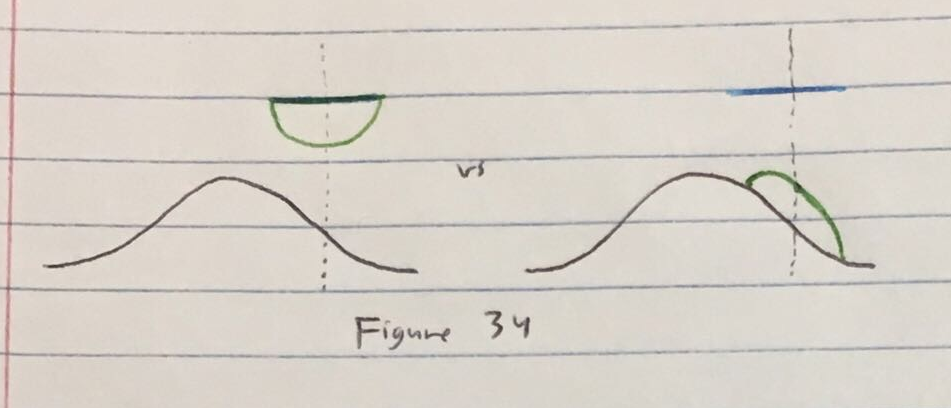
\includegraphics[width=\fw]{img/10-constructed/02.png}
  \caption{Caption}
\end{figure}

But one day a cool idea occurred to me. Instead of lowering a half-circle towards the function $y = f(x)$, why don't we just (for every $x \in [x_o - N, x_o + N]$), \textit{add} the exact vertical thickness of that half-circle \textit{to} the function down below, giving it a sort of raised bump shape on top on interval $[x_o - N, x_o + N]$. In so doing, we can reduce the fairly nasty problem of lowering half a circle down towards the function to a much simple problem of lowering a straight horizontal line down towards the function + bump. And when will the horizontal line first contact it?

At the maximum of course! The value of $y_c$ which first makes contact it $y_c = max \{ f(x) + \sqrt{ N^2 - (x - x_o)^2 } | x \in [ x_o - N, x_o + N] \}$.

When $N$ is negative, we are below the function and so we must \textit{subtract} a semi-circular bump from beneath the function instead. Putting this all together, we arrive at the following conclusion:

\begin{theorem}

  A nice simple formula for the $y$-value at the Snipped $N$-Units Away Curve at $x_o$ is
  \begin{center}
    $
    f_N(x_o) =
    \begin{cases}
    % case 1
      % expression
      max \{ f(x) + \sqrt{ N^2 - (x - x_o)^2 } | x \in [ x_o - N, x_o + N] \}, &
      % condition
      N > 0 \\
    % case 2
      % expression
      min \{ f(x) - \sqrt{ N^2 - (x - x_o)^2 } | x \in [ x_o - N, x_o + N] \}, &
      % condition
      N < 0
    \end{cases}
    $
  \end{center}

\end{theorem}

Let's give an example of how to use this tool. Pick a function, how about a classical $y = sin x$?. Choose an $N$ value, maybe $N = 2$. Lastly choose a value of $x_o$, maybe $x_o = 2.5$. These choices are depicted in Figure $\ref{constructed:3}$. How do we find the $y$-value of the Snipped $N$-Units Away Curve at $x = x_o$? We can see it in (Fig $\ref{constructed:3}$...

How does one find that? The theorem guarantees us that $f_N(x_o) = max \{ f(x) + \sqrt{ N^2 - (x - x_o)^2 } | x \in [ x_o - N, x_o + N ] \} = max \{ sin x + \sqrt{ 4 - (x - 2.5)^2 } | x \in [ \dfrac{1}{2}, \dfrac{9}{2} ] \}$. We computer-approximate this using a Graphic Calculator in Figure $\ref{constructed:4}$ to gather that the maximum value $\approx 2.8542$. Adding to the plot in Figure $\ref{constructed:3}$ the function $y = 2.8542$ shows that our formula is spot on...

\renewcommand\w{0.3\linewidth}
\renewcommand\fw{0.9\textwidth}

\begin{figure}[h]
  \centering
  \begin{minipage}[b]{\w}
    \centering
    \label{constructed:3}
    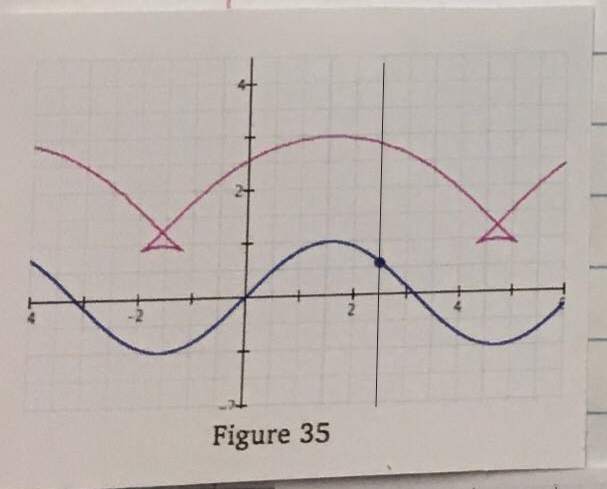
\includegraphics[width=\fw]{img/10-constructed/03.png}
    \caption{Caption}
    \vspace{4ex}
  \end{minipage} % end
  \begin{minipage}[b]{\w}
    \centering
    \label{constructed:4}
    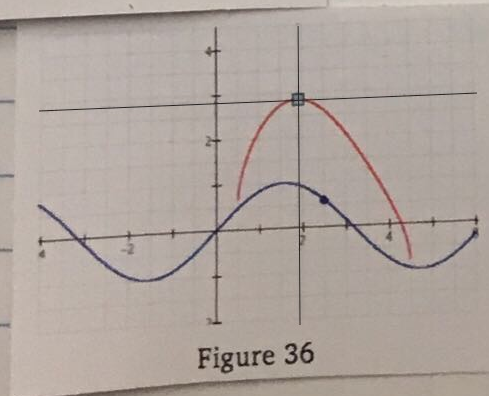
\includegraphics[width=\fw]{img/10-constructed/04.png}
    \caption{Caption}
    \vspace{4ex}
  \end{minipage} % end
  \begin{minipage}[b]{\w}
    \centering
    \label{constructed:5}
    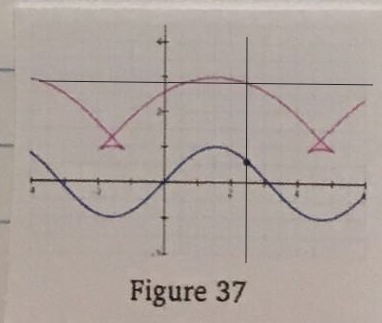
\includegraphics[width=\fw]{img/10-constructed/05.png}
    \caption{Caption}
    \vspace{4ex}
  \end{minipage} % end
\end{figure}

  \section{A Beautiful Observation}

This idea occurred to me one day on a public bus in downtown Rochester. Take a function $y = f(x)$ and find one of its values of $x$ that coincides with a minimum of $R(x)$, the radius of curvature for the function. Call that value $x_m$. We know from the theorem is section 9 that the function $y = f(x)$ will spawn a crunch spot from precisely that value of $x$. The crunch spot will occur for the ``critical value'' of $N = \dfrac{f''(x_m)}{|f''(x_m)|} R(x_m)$. But by the definition of radius of curvature, we know that on some potentially small neighborhood of $x_m, y = f(x)$ will approximate an arc of a circle of radius $R(x_m)$ whose center is that crunch spot. Take in your imagination this brief circle arc. If we send forth from each point along that arc a normal line, we know they all converge at the crunch spot. This means no matter what we set $N$ to positive or negative, that the $N$-Units Away Curve spots generated by the part of $y = f(x)$ that approximates a circle will also approximate a circle! This gives us the fascinating result that the ``bottom'' of each divot triangle has a shape approximately a circular arc. This is a very strange, beautiful result and is depicted in Figures $\ref{beautiful:1}$ and $\ref{beautiful:2}$ bellow:

\renewcommand\w{0.9\linewidth}
\renewcommand\fw{0.9\textwidth}
\renewcommand\fh{0.25\textheight}

\begin{figure}[H]
  \centering
  \begin{minipage}[b]{\w}
    \centering
    \label{beautiful:1}
    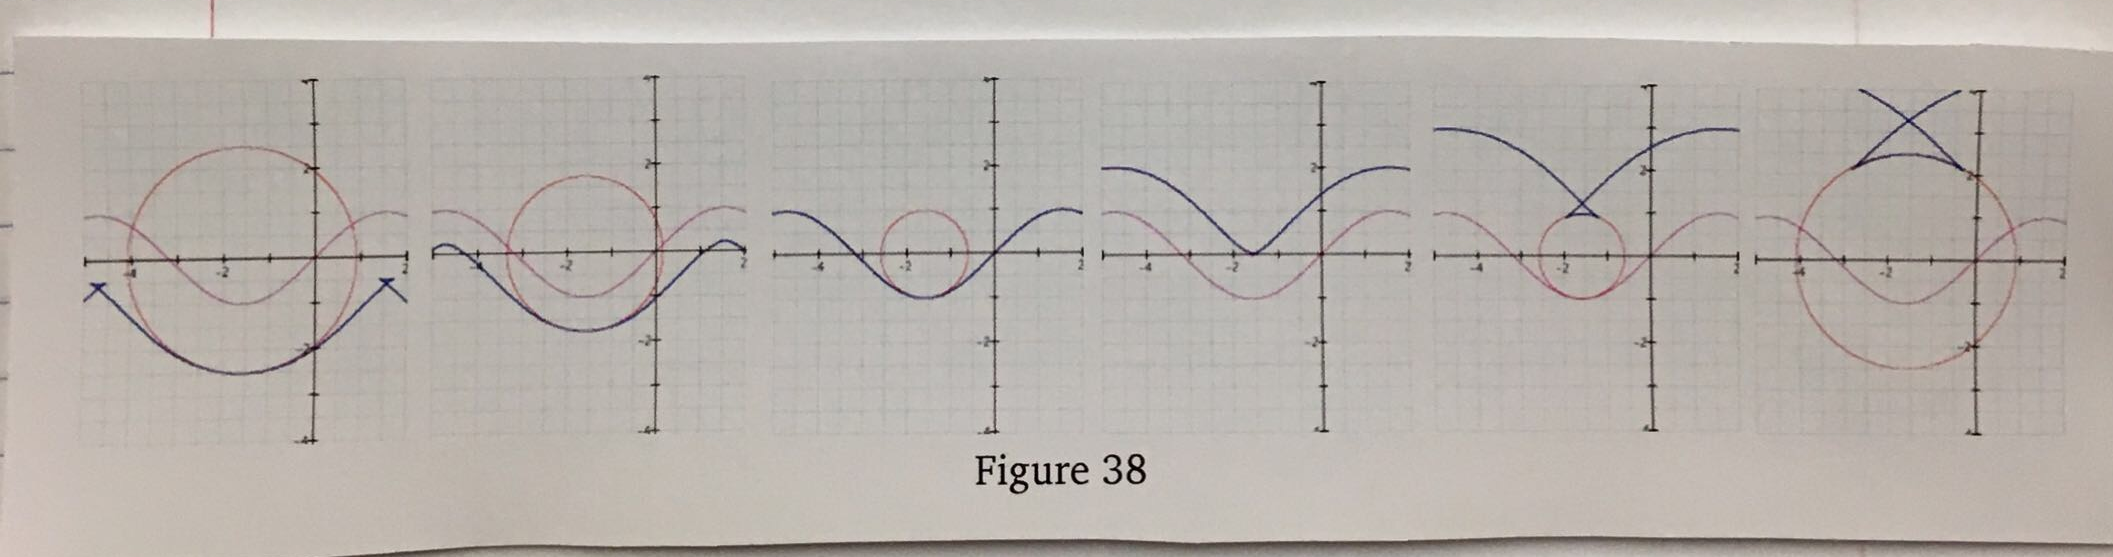
\includegraphics[width=\fw, height=\fh, keepaspectratio]{img/11-beautiful/01.png}
    \caption{Caption}
    \vspace{4ex}
  \end{minipage}
  \begin{minipage}[b]{\w}
    \centering
    \label{beautiful:2}
    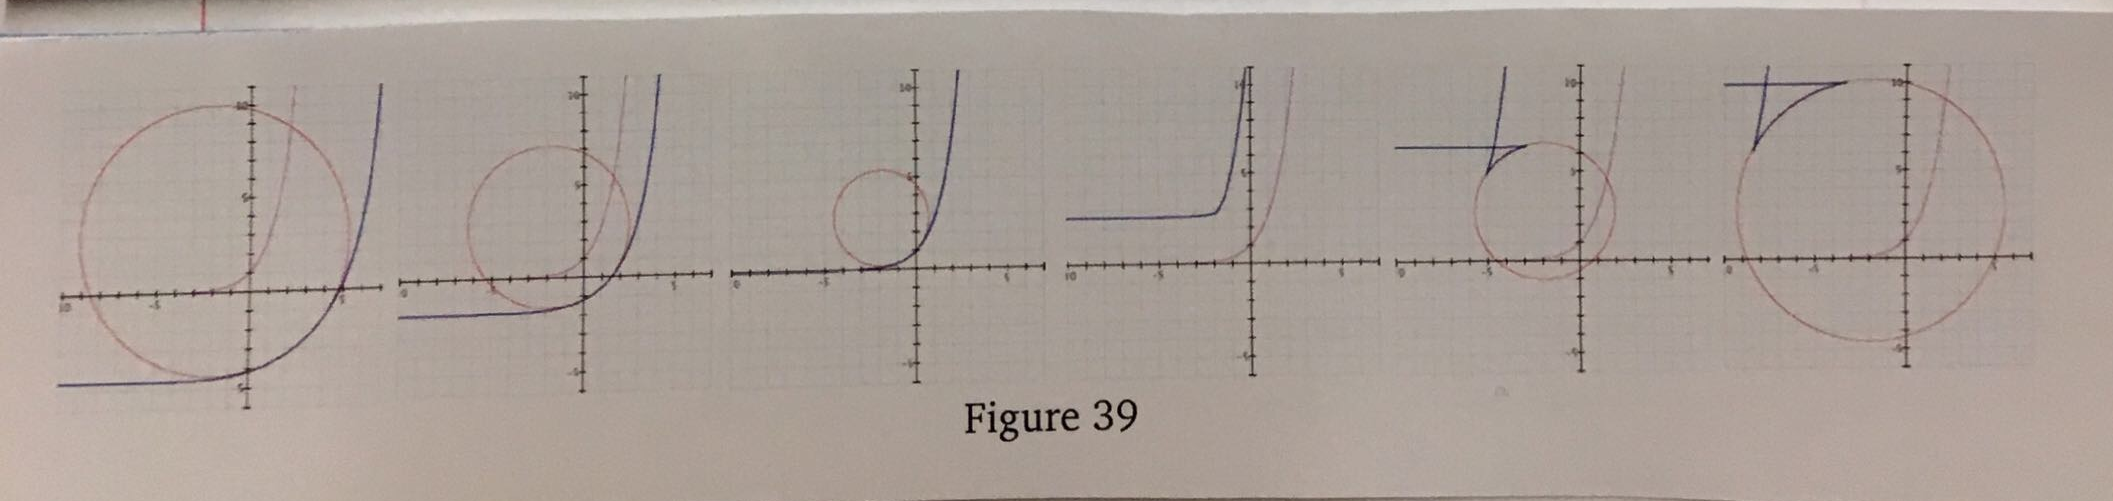
\includegraphics[width=\fw, height=\fh, keepaspectratio]{img/11-beautiful/02.png}
    \caption{Caption}
    \vspace{4ex}
  \end{minipage}
\end{figure}

  \section{Solving Divot Paths}

\renewcommand\w{0.25\textwidth}
\renewcommand\fw{0.9\linewidth}

\begin{wrapfigure}{l}{\w}
  \label{divot:1}
  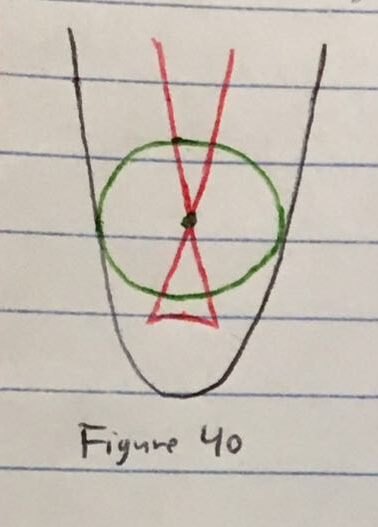
\includegraphics[width=\fw]{img/12-divot/01.png}
  \caption{Caption}
\end{wrapfigure}


In trying to map out the science of the $N$-Units Away Curves, by far the most difficult, enigmatic portion of it all is the science of Divot Triangles. Where do they go as $N$ increases? For the last many months I have been consumed by that mystery. I'm very proud to have finally solved it and put it to rest.

Recall from section 9 that the apex of each divot triangle is precisely where a marble rolling along the curve would get stuck, the $N$-Units Away Curve travelling further to the right into an ?? of the function to tight for the marble to follow into. At some point the $N$-Units Away Curve heads back to the left (it must if it is to re-arrive at the divot triangle apex). It passes underneath the apex and finally turns around again at the other divot triangle base point. We see that the divot base points occur that those values of $t$ at which the horizontal motion of the $N$-Units Away Curve changes direction, aka when $x_N(t)$ achieves a local min or a local max. This concept is plotted in Figures and with $x_N(t = x)$ plotted in green.

\renewcommand\w{0.4\textwidth}
\renewcommand\fw{0.9\linewidth}
\renewcommand\fh{.25\textheight}

\begin{figure}[H]
  \centering
  \begin{minipage}[b]{\w}
    \label{divot:2}
    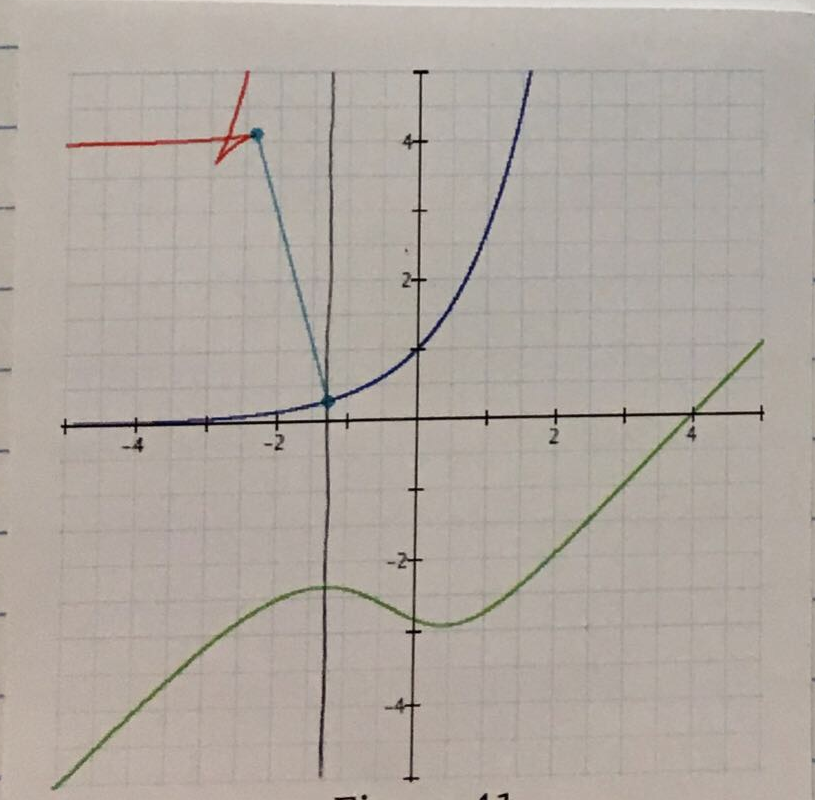
\includegraphics[width=\fw, height=\fh, keepaspectratio]{img/12-divot/02.png}
    \caption{Caption}
  \end{minipage}
  \begin{minipage}[b]{\w}
    \label{divot:3}
    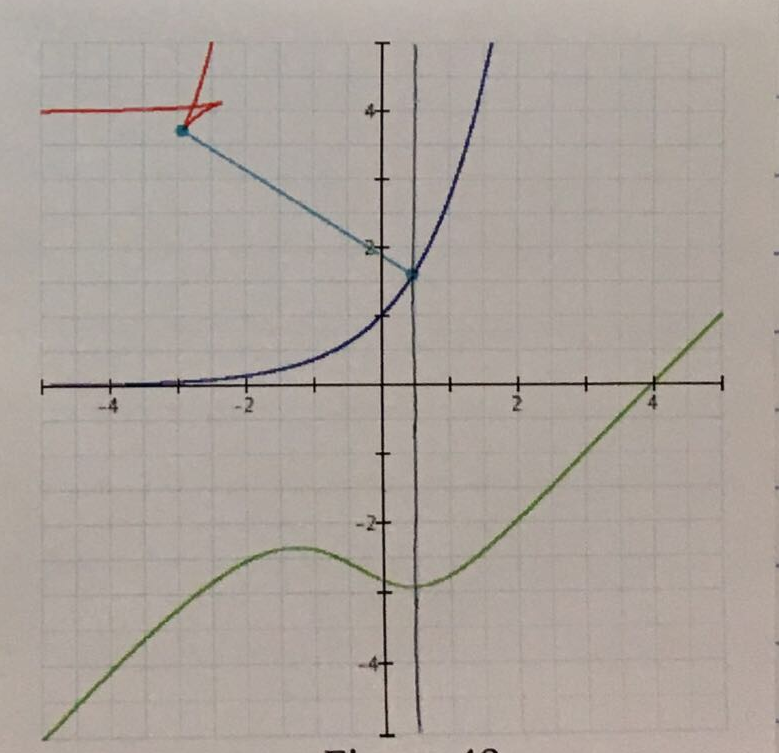
\includegraphics[width=\fw, height=\fh, keepaspectratio]{img/12-divot/03.png}
    \caption{Caption}
  \end{minipage}
\end{figure}

\renewcommand\bvec{\langle -f'(t), 1 \rangle}

So to find the base points of the divot triangle, we must find the zeros of $x_N'(t)$. $x_N(t) = t - N \dfrac{f'(t)}{| \bvec |} = t - N f'(t) ( (f'(t))^2 + 1 ) ^ { -1/2 }$, so $x_N'(t) = 1 - N f''(t) ( (f'(t))^2 + 1 ) ^ { -1/2 } + N f'(t) ( (f'(t))^2 + 1 ) ^ { -1/2 } ( f'(t) f''(t) )$. But setting this equal to zero and trying to solve for $t$ is an exercise in madness! It becomes a complete and total mess.

However, recall from section 8 that we proved $y_N'(t) = f'(t) x_N'(t)$. Thus one way to solve for zeros of $x_N'(t)$ is tp solve for the zeroes of $y_N'(t)$ instead! We might occasionally find that $y_N'$ is 0 when $x_N'$ is not due to $f'(t)$ being 0. but we can simply brush aside those case when $f'(t) = 0$, the original curve and also the $N$-Units Away Curve are ?? approximating a flat horizontal line at that $t$-value. There can be no divot triangle bases at such a spot.

Assuming $f'(t) \neq 0$, when is $y'(t) = 0$?

\begin{align*}
% line 1
  f'(t) - \dfrac{N}{2} f'(t) ((f'(t))^2 + 1) ^ {-3/2} (2 f'(t) f''(t)) = 0, &
  &
  % reasoning
  \text{ (established in section 8) } \\
% line 2
  f'(t) = N (f'(t))^2 f''(t) ( (f'(t)^2 + 1 ) ^ {-3/2} \\
% line 3
  1 = N f'(t) f''(t) ( (f'(t)^2 + 1 ) ^ {-3/2}, &
  &
  % reasoning
  \text{ since $f'(t) \neq 0$, we can divide both sides by it } \\
% line 4
  ( (f'(t))^2 + 1 ) ^ {3 / 2} = N f'(t) f''(t), &
  &
  % reasoning
  \text{ multiply both sides by $((f'(t) ^ 2 + 1) ^ {3 / 2}$ }
\end{align*}

This fact will be true for every $t$-value that acts as a divot triangle base point. So what happens as $N \xrightarrow{} \infty$? How can this equality remain valid?

Take some sequence of $(N, t)$ pairs $((N_j, t_j))_{ j \geq 1}$, with $N_j \xrightarrow{} \infty$ as $j \xrightarrow{} \infty$. As $N_j \xrightarrow{} \infty$, what must $t_j$ do to keep the above valid?

If the $LHS$ also $\xrightarrow{} \infty$, then $((f'(t_j))^2 + 1) ^ {3/2} \xrightarrow{} \infty \implies f'(t_j) \xrightarrow{} \infty$.

There's our first possibility.

If the $LHS$ does \textit{not} $\xrightarrow{} \infty$, then something on the $RHS$ must be going to 0 to hold $N$ back. We know it cannot be that $f'(t_j) \xrightarrow{} 0$, as stated above, this would guarantee that we are approaching a flat horizontal part of the curve which would not be creating a divot base point. It must be that $f''(t) \implies 0$! This is out other possibility.

Figure $\ref{divot:4}$ shows a plot of the $t$ values corresponding to the divot triangle base points for the function $y = e^x$. Our theory predicts that a $N \xrightarrow{} \infty$ the $t$-values necessarily approach either $f'(t) \xrightarrow{} \infty$ (so the positive $t$-value here should slowly work its way towards infinity) or $f''(t) \xrightarrow{} 0$ (so the negative $t$-value here should work its way towards negative infinity. Figure $\ref{divot:4}$ presents $N = 5, 50, 500$.

\renewcommand\w{0.9\textwidth}
\renewcommand\fw{0.9\linewidth}
\renewcommand\fh{.25\textheight}

\begin{figure}[H]
  \centering
  \begin{minipage}[b]{\w}
    \label{divot:4}
    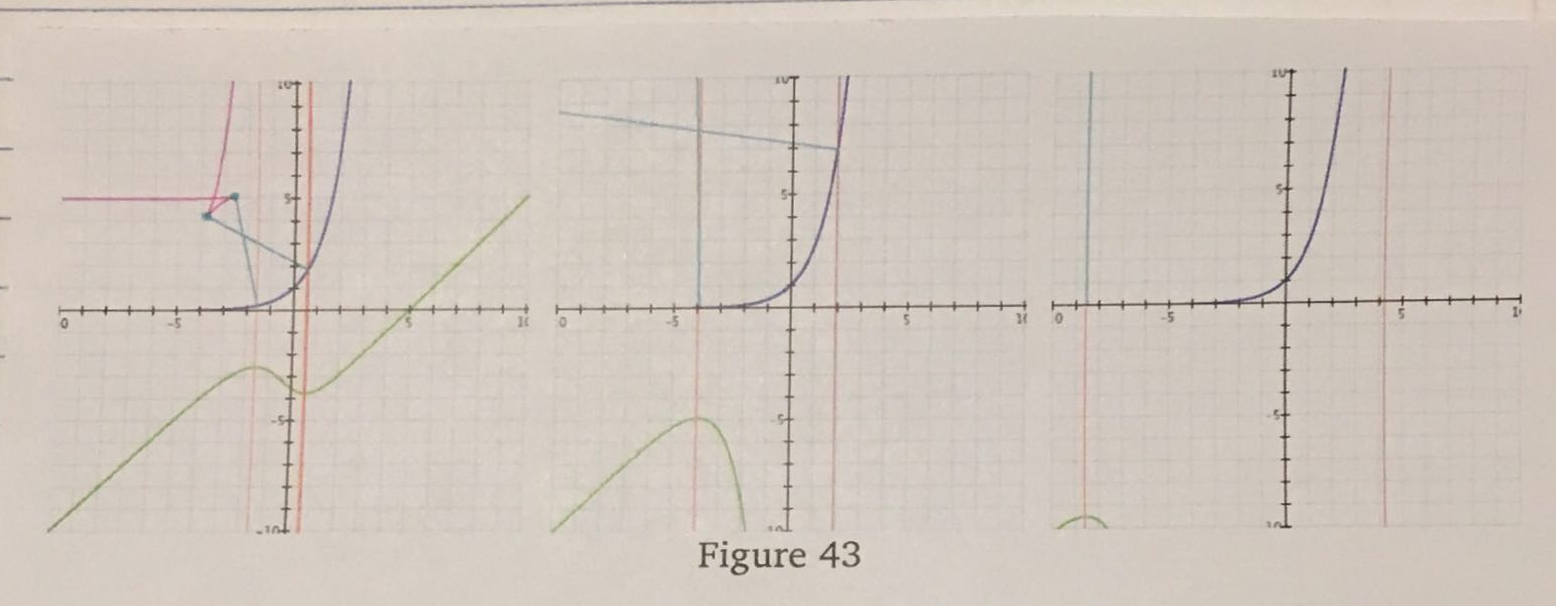
\includegraphics[width=\fw, height=\fh, keepaspectratio]{img/12-divot/04.png}
    \caption{Caption}
  \end{minipage}
\end{figure}

Figure $\ref{divot:5}$ shows a plot of the $t$ values corresponding to the divot triangle base points for the function $y = e^{-x^2}$ Our theory predicts that as $N \xrightarrow{} \infty$, the $t$-values necessarily must approach either $f'(t) \xrightarrow{} \infty$ (which does not occur here), or $f''(t) \xrightarrow{} 0$. Figure $\ref{divot:5}$ also plots in light blue the double derivative $f''$, offering a more clear understanding of what it means for these $t$ values to chase after occurrences of $f''(t) \xrightarrow{} 0$. Figure $\ref{divot:5}$ presents $N = 5, 500, 5000000$.

\renewcommand\w{0.9\textwidth}
\renewcommand\fw{0.9\linewidth}
\renewcommand\fh{.25\textheight}

\begin{figure}[H]
  \centering
  \begin{minipage}[b]{\w}
    \label{divot:5}
    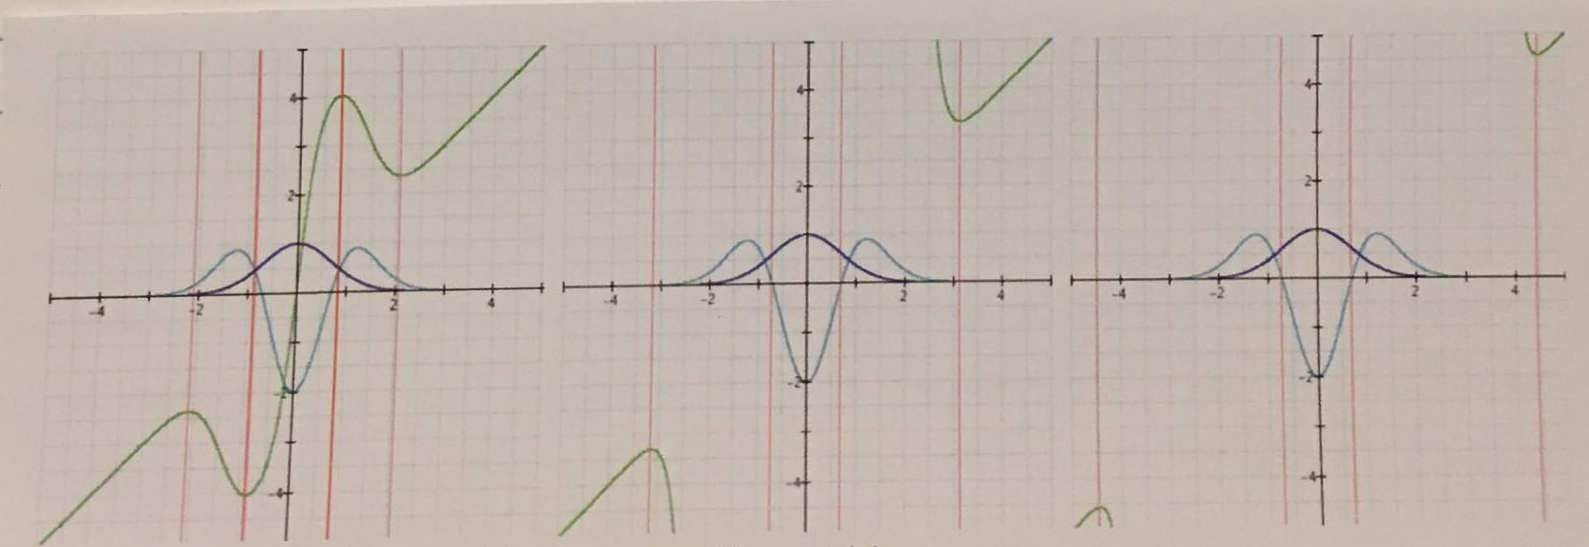
\includegraphics[width=\fw, height=\fh, keepaspectratio]{img/12-divot/05.png}
    \caption{Caption}
  \end{minipage}
\end{figure}

This understanding of where $t$-values that generate the divot triangle base points are moving lets us intelligently discuss where the triangle base points are going as $N \xrightarrow{} \infty$.

\renewcommand\w{0.25\textwidth}
\renewcommand\fw{0.9\linewidth}

\begin{wrapfigure}{l}{\w}
  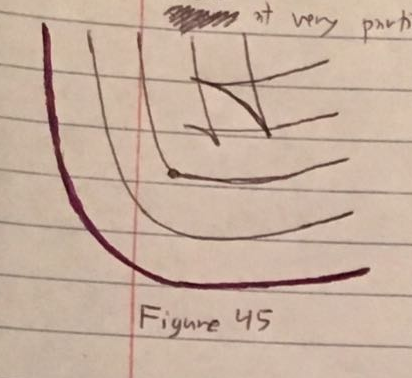
\includegraphics[width=\fw]{img/12-divot/06.png}
  \caption{Caption}
  \label{divot:6}
\end{wrapfigure}

Now we move on in our discussion to the science of divot triangle apex points. Take some function $y = f(x)$ twice differentiable whose second derivative is continuous.  When $N$ is 0, $f_N(t)$ will have no crunch point. If you begin raising or lowering the value of $N$, however, so long as $f(x)$ has any twists or turns at all and is not a perfectly straight line on all $x \in \mathbb{R}$. we will find crunch spots. These will occur at very particular values of $N$, spawning the birth of divot triangles.

We've shown that you can view the $N$-Units Away Curves as being the paths that the centerpoint of marbles of radius $N$ would take as they rolled along the function. The marbles get stuck on their travels precisely at the apex points of the divot triangles, as those are the values of the $N$-Units Away Curves that have \textit{two} values $t$ associated with those points, meaning a marble would contact the original function $y = f(x)$ at two points there, thus being held in place. Consider the example of $y = x^2$ (Fig $\ref{divot:7}$. We see that as $N$ increases, the apex of the divot triangles follow a very specific path through $\mathbb{R}^2$. You could view that path as the centerpoints of a while succession of stuck marbles, each with slightly larger radius than the last. The very lowest one has its centerpoint exactly at the crunch spot.

It's almost as if we've taken the ``initial ball'' we'll call it, the one centered at the crunch spot, ans swelled it to a larger radius. We've then plotted where that swelling ball will go as it gets bigger. As the little initial ball is inflated to get bigger and bigger, surely its centerpoint must move further and further from the original function $y = f(x)$. Let's go about this n the following manner...

\renewcommand\w{0.4\textwidth}
\renewcommand\fw{0.9\linewidth}
\renewcommand\fh{0.2\textheight}

\begin{figure}[H]
  \centering
  \begin{minipage}[b]{\w}
    \centering
    \label{divot:7}
    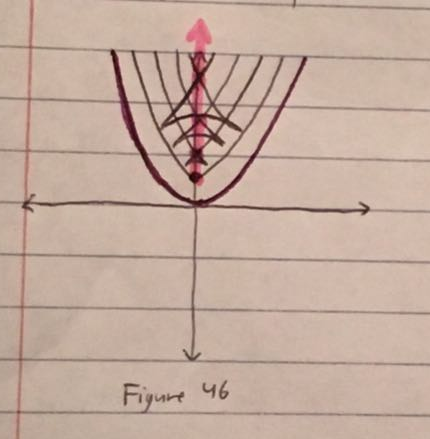
\includegraphics[height=\fh]{img/12-divot/07.png}
    \caption{Caption}
  \end{minipage}
  \begin{minipage}[b]{\w}
    \centering
    \label{divot:8}
    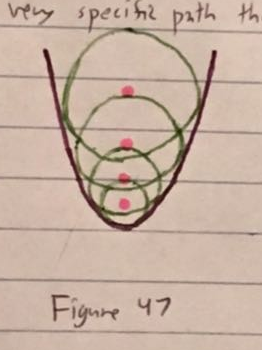
\includegraphics[height=\fh]{img/12-divot/08.png}
    \caption{Caption}
  \end{minipage}
\end{figure}

Choose a function $y = f(x)$. Find a crunch spot for that function.

\renewcommand\w{0.25\textwidth}
\renewcommand\fw{0.9\linewidth}

\begin{wrapfigure}{l}{\w}
  \label{divot:9}
  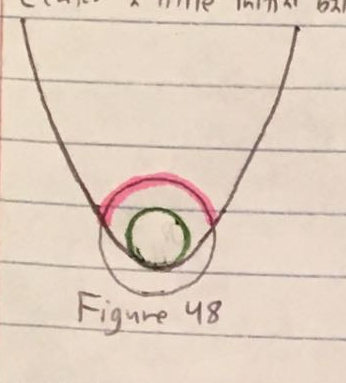
\includegraphics[width=\fw]{img/12-divot/09.png}
  \caption{Caption}
\end{wrapfigure}

Center a little initial ball at the crunch spot and give it the critical value of $N$, call it $N_o$, as its radius (Fig $\ref{divot:9}$. That crunch spot is exactly where the divot triangle apex path begins. But where does it go as $N$ increases? Choose some $r > 0$. Draw another circles centered at the crunch spot but give this one radius $N_o + r$. As $N$ increases, the divot apex must rise up and away from the function (as it effectively represents where larger and larger marbles of radius $N$ will get stuck), thus the divot apex path must cross the new circle at some point. Assuredly the divot apex path cannot suddenly go \textit{below} the function $y = f(x)$, so for now highlight the area of the new circle that lies above the function $y = f(x)$.

\renewcommand\w{0.25\textwidth}
\renewcommand\fw{0.9\linewidth}

\begin{wrapfigure}{l}{\w}
  \label{divot:10}
  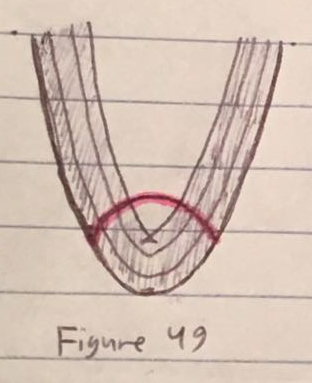
\includegraphics[width=\fw]{img/12-divot/10.png}
  \caption{Caption}
\end{wrapfigure}

These are our ``suspect''. Re-draw this little highlighted region and consider just it now. (Fig $\ref{divot:10}$. Take this set up and now begin drawing some of the function's $N$-Units Away Curves, starting at first with very small $ \Delta N$. ``Grey out'' any areas of $\mathbb{R}^2$ that lie between $y = f(x)$ and these $N$-Units Away Curves. You could think of these almost like little waces washing away more and more of the highlighted region. Figure $\ref{divot:11}$ shows that some point the $\Delta N$ has washed away all of the highlighted region aka ``the suspects''.

\renewcommand\w{0.25\textwidth}
\renewcommand\fw{0.9\linewidth}

\begin{wrapfigure}{l}{\w}
  \label{divot:11}
  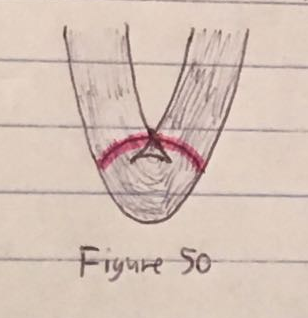
\includegraphics[width=\fw]{img/12-divot/11.png}
  \caption{Caption}
\end{wrapfigure}

Whichever point of the highlighted region is left appears to be a divot apex point. Note that it is also the highlighted point that lay furthest from $y = f(x)$. This leads us to the following conjectural observation: Where the Divot Apex point crosses that little highlighted region appears to be precisely at the point of the highlighted region which lies furthest from $y = f(x)$.

\renewcommand\w{0.25\textwidth}
\renewcommand\fw{0.9\linewidth}

\begin{wrapfigure}{l}{\w}
  \label{divot:12}
  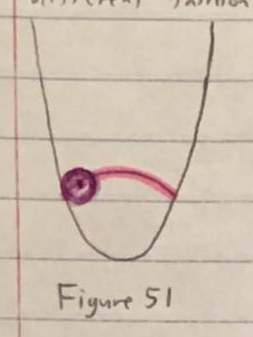
\includegraphics[width=\fw]{img/12-divot/12.png}
  \caption{Caption}
\end{wrapfigure}

Consider back to figure $\ref{divot:8}$ of the idea that the divot apex points represent precisely where marble of larger and larger radii would get stuck. Let's reconsider that idea in a slightly different fashion. Draw a function $y = f(x)$. Fins an initial ball and draw a slighlty larger circle arounf it. Highlight the points above $y = f(x)$. These are our ``suspects'' for where the divot apex passes through. We know it travels through at least one of these spots. Pick a spot very far to the left on this little arc (Fig $\ref{divot:12}$. Draw the largest circle you centered there which does not cross $y = f(x)$. This cannot be the divot apex point, as were we to increase $N$ slowly and draw $N$-Units Away segment, never being contacted at all by the right sick. The divot apex point must be \textit{equidistant} from $y = f(x)$ on both sides! That's how a marble can get stuck there. How can we find a point on this highlighted region which is equidistant from both sides? Find the part of the highlighted arc which is furthest from $y = f(x)$ altogether! We know it will be equidistant from both sides, as if you move from it in either direction you're come closer to the function. How do we go about finding which point of the highlighted arc is furthest from the function?

Let us construct a specialized function specifically for this job. The distance between any two points $(x_0, y_0)$ and $(x_1, y_1)$ is $d = \sqrt{ (x_0 - x_1)^2 + (y_0 - y_1)^2 }$, Thus if we want to know how far away any arbitrary points of $\mathbb{R}^2$ $(x_0, y_0)$ is from a function $y = f(x)$. we can see that it is $D_{y = f(x)}(x_0, y_0) = min \{ \sqrt{ (x_0 - x_1)^2 + (y_0 - y_1)^2 } | x \in \mathbb{R}^2$,

\renewcommand\w{0.25\textwidth}
\renewcommand\fw{0.9\linewidth}

\begin{wrapfigure}{l}{\w}
  \label{divot:13}
  \includegraphics[width=\fw]{img/12-divot/13.png}
  \caption{Caption}
\end{wrapfigure}

This $D$ is a function of two variables, a scalar field if you will, which assigns to every point of $\mathbb{R}^2$ a value ``how far is this point from the function''. As we take the ``initial ball'' and swell it, it gets lifted up and away from the function, its centerpoint (aka the Divot Apex point) travelling up and up following the route of whatever location maximizes distance from $y = f(x)$! If $F_{f(x)} (x_0, y_0)$ is a scalar field, the Divot Apex point is following the gradient of this field!

We can use this knowledge to finally address the question stated in section 3 of why does the divot apex point above the curve $y = x^3$ seem to follow a path that sweeps out to the left? Check this out...

\renewcommand\w{0.25\textwidth}
\renewcommand\fw{0.9\linewidth}

\begin{wrapfigure}{l}{\w}
  \label{divot:14}
  \includegraphics[width=\fw]{img/12-divot/14.png}
  \caption{Caption}
\end{wrapfigure}

\begin{enumerate}
  \item Draw the function $y = x^3$
  \item Plot a crunch spot
  \item Surrounding that crunch spot, draw a good number of concentric circles of various radii and highlight the portions of them that are on the same side of $y = f(x)$ at the crunch spot.
  \item Mark on these highlighted arcs the points which are local maximums of $D_{x^3} (x_0, y_0)$ aka which points are furthest from the function.
  \item Draw a line connecting the crunch spot through these locations of maximum distance from $y = f(x)$, and voila! You have your divot apex path.
\end{enumerate}

The divot apex path starts at the crunch spot and follow the gradient of $D_{f(x)} (x_0, y_0)$, seeking for every $\Delta N$ location on $\mathbb{R}^2$ further and further distant from $y = f(x)$.

This concludes the main discussions of this paper.

  \section{Applications Part One - Railroads}

So while working on this topic, I kept thinking to myself: What practical applications does this theory have out in the real world? Where in science/nature/technology do we spot $N$-Units Away Curves? The first immediate thought that comes to my mind is railroad tracks.

The left rail of a railroad track is set to be exactly the same consistent distance away from the right rail at all locations. You literally have two curves that remain some fixed $N$-Units Away from one another at all spots! This is what lets a train of fixed width ride along it smoothly.

So considering that my $N$-Units Away Theory is brand new and yet trains have been driving on tracks since the early 1800's, I was instantly stuck with the question: How is it that railroad engineers have been building fairly spot on approximations of $N$-Units Away Curves for all these years?

I did some significant research into the topic, assisted greatly by a book I found called \textit{Railroad Engineering} by William W. Hay, and discovered the truly improbable, ridiculous, and highly enjoyable answer. When railroad engineers first want to lay down a railroad track through a new area, first they prepare a track bed for the train. Sometimes this means digging a trench for a train track. More often it just means clearing away debris / trees and making the ground level along the desired route. Next they unload 60 foot long prefabricated track pieces (the underlying supportive cross beams that the rails will sit atop). Finally they lay down long long bendy rail strips on top made of a high quality steel alloy. They place these rail strips down onto the cross beams sorta any which way. The distance between them at this stage doesn't really matter. They’re all higgledy-piggledy. It’s the furthest thing from a nice approximation of $N$-Units Away Curves. How do they then get from that to the nice $N$-Units Away Curves-like final product?

They use an amazing device called a Rail Threader! It operates like a gigantic zipper. It has highly flexible wheels and can roll along the highly unevenly distant-from-each-other rails. Periodically it pauses, puts down two large hydrolic ``feet'' and lifts off the ground, taking the flexible rails with it about a foot into the air. It then moves them laterally to the exact desired standard gauge distance the rails should be from one another and places them down. We now have a beautiful approximation of an $N$-Units Away Curve which the railroad crews then bolt down into place. The Rail Threader acts like a zipper, taking in the higgledy-piggledy rails and leaving behind it as it goes a nice perfect Standard-Gauge N-Units Away Curves track. Absolutely amazing! A real ``engineer's answer'' to an otherwise very tricky math problem.

\renewcommand\w{0.3\linewidth}
\renewcommand\fw{0.9\textwidth}

\begin{figure}[h]
  \centering
  \begin{minipage}[b]{\w}
    \centering
    \includegraphics[width=\fw]{img/13-app/01.png}
    \caption{Caption}
    \vspace{4ex}
  \end{minipage} % end
  \begin{minipage}[b]{\w}
    \centering
    \includegraphics[width=\fw]{img/13-app/02.png}
    \caption{Caption}
    \vspace{4ex}
  \end{minipage} % end
  \begin{minipage}[b]{\w}
    \centering
    \includegraphics[width=\fw]{img/13-app/03.png}
    \caption{Caption}
    \vspace{4ex}
  \end{minipage} % end
\end{figure}

  \section{Applications Part Two - Optics}

It was my classmate friend Dustin Kesler who looked over at me one day and said the phrase, ``Wait a minute. These $N$-Units Away Curve crunch spots... Don’t they look kinda like a focal point to you?'' It began us thinking about $N$-Units Away Curves in a whole new way and really brought up the question – is there any connection between $N$-Units Away Curves and Optics?

I ended up having two interviews with people in the University of Rochester Optics Department, one with an undergrad friend of mine Mike Taylor, one with a senior researcher named Professor Jannick Rolland. Speaking with these profound optics minds, a few fascinating things become readily clear. When you think of an $N$-Units Away Curve drifting steadily further and further from a function $y = f(x)$, what is really going on is highly akin to a wave propagating through space.

Obscure though it might be, consider owning a stereo speaker shaped exactly like the function $y = sin(x)$. When it blasts a musical note, the shape of that soundwave travelling through the air will take on the exact shape of our $N$-Units Away Curves travelling on the $\mathbb{R}^2$ plane as $N$ increases! What a profound and different way to think about $N$-Units Away Curves... as wave propagation!

\renewcommand\fw{0.9\linewidth}

\begin{figure}[h]
  \centering
  \label{constructed:2}
  \includegraphics[width=\fw]{img/13-app/04.png}
  \caption{Caption}
\end{figure}

Consider on the other hand using a 3D printing machine to make a little plastic version of the function $y = sin(x)$. Make it perfectly exacting in shape but incredibly thin, almost wire thin. Now imagine walking to a perfectly still body of water (maybe a bath tub) and dropping the y=sin(x) shaped piece into the water horizontally so it all hits the surface at the exact same time. Can you guess what shape the resultant wave will be as it drifts away from $y = sin(x)$? Why it will perfectly resemble an $N$-Units Away Curve for that function!

I found this utterly fascinating and am very much so hoping to someday perform this exact experiment. I hope to film the whole thing with a nice high-speed camera and take a careful look at real world $N$-Units Away Curves!! How profoundly interesting. I didn't use to have any idea that these theoretical math constructions of mine had a role in the physical reality around us. To be honest, my question about said bath-tub $y = sin(x)$ wave experiment is the following: When the wave collapses upon itself at the crunch spots, probably one of two things will occur. Either we’ll see perfect nice little divot triangles form, exactly as in $N$-Units Away Theory, or we’ll see the water right in that area respond chaotically with turbulence instead. It’s very much so a question open for debate! In the real world, when you spot an $N$-Unit Away Curve, do the crunch spots create divot triangles or turbulence?

I leave that for my reader as a mystery for another day.

  \renewcommand\figuresI{

  \renewcommand\w{0.4\linewidth}
  \renewcommand\fw{0.9\textwidth}

  \begin{figure}[H]
    \begin{minipage}[b]{\w}
      \centering
      \label{parametric:2}
      \includegraphics[width=\fw]{img/15-parametric/02.png}
      \caption{Caption}
      \vspace{4ex}
    \end{minipage} % end
    \begin{minipage}[b]{\w}
      \centering
      \label{parametric:3}
      \includegraphics[width=\fw]{img/15-parametric/03.png}
      \caption{Caption}
      \vspace{4ex}
    \end{minipage} % end
    \begin{minipage}[b]{\w}
      \centering
      \label{parametric:4}
      \includegraphics[width=\fw]{img/15-parametric/04.png}
      \caption{Caption}
      \vspace{4ex}
    \end{minipage} % end
    \begin{minipage}[b]{\w}
      \centering
      \label{parametric:5}
      \includegraphics[width=\fw]{img/15-parametric/05.png}
      \caption{Caption}
      \vspace{4ex}
    \end{minipage} % end
    \begin{minipage}[b]{\w}
      \centering
      \label{parametric:6}
      \includegraphics[width=\fw]{img/15-parametric/06.png}
      \caption{Caption}
      \vspace{4ex}
    \end{minipage} % end
  \end{figure}

}

\renewcommand\figuresII{

  \renewcommand\w{0.4\linewidth}
  \renewcommand\fw{0.9\textwidth}

  \begin{figure}[H]
    \centering
    \begin{minipage}[b]{\w}
      \centering
      \label{parametric:7}
      \includegraphics[width=\fw]{img/15-parametric/07.png}
      \caption{Caption}
      \vspace{4ex}
    \end{minipage} % end
    \begin{minipage}[b]{\w}
      \centering
      \label{parametric:8}
      \includegraphics[width=\fw]{img/15-parametric/08.png}
      \caption{Caption}
      \vspace{4ex}
    \end{minipage} % end
    \begin{minipage}[b]{\w}
      \centering
      \label{parametric:9}
      \includegraphics[width=\fw]{img/15-parametric/09.png}
      \caption{Caption}
      \vspace{4ex}
    \end{minipage} % end
    \begin{minipage}[b]{\w}
      \centering
      \label{parametric:10}
      \includegraphics[width=\fw]{img/15-parametric/10.png}
      \caption{Caption}
      \vspace{4ex}
    \end{minipage} % end
  \end{figure}

}

\newcommand{\finalFormula}{


}

\section{The Parametric Case and the Polar Case}

Suppose you want to study the $N$-Units Away Curves of a curve, but you do not have it in a simple closed $y = f(x)$ form but instead you have a parametric function $
\begin{bmatrix}
  x(t) \\
  y(t)
\end{bmatrix} =
\begin{bmatrix}
  g(t) \\
  h(t)
\end{bmatrix} $. Can you still find the $N$-Units Away Curves to that parametric curve in $\mathbb{R}^2$?

I had always hoped I might be able to solve for the $N$-Units Away Curves in the case, and in fact I have been able to! So long as functions $g$ and $h$ are differentiable.

Take some value of $t$. Call it $t_o$. The slope of the parametric curve at location $t = t_o$ is $ \dfrac{dy}{dx} =
\dfrac{\dfrac{dy}{dt}}{\dfrac{dy}{dt}} = \dfrac{y'(t)}{x'(t)} = \dfrac{h'(t)}{g'(t)} $. Take note, of course, that this formula is only valid so long as $g'(t) \neq 0$. Suspend your disbelief for the moment and simply ignore those values of $t$. The final formula will address them.

Where before we had: $\begin{bmatrix} x \\ y \end{bmatrix} = \begin{bmatrix} t \\ f'(t) \end{bmatrix} + N \dfrac{\begin{bmatrix} -f'(t) \\ 1 \end{bmatrix}}{|\begin{bmatrix} -f'(t) \\ 1 \end{bmatrix}|}$, now replace every occurrence of $f'(t)$ with $\dfrac{h'(t)}{g'(t)}$ to get $\begin{bmatrix} x \\ y \end{bmatrix} = \begin{bmatrix} 1 \\ \dfrac{h'(t)}{g'(t)} \end{bmatrix} + N \dfrac{\begin{bmatrix} \dfrac{-h'(t)}{g'(t)} \\ 1 \end{bmatrix}}{\left| \begin{bmatrix} \dfrac{-h'(t)}{g'(t)} \\ 1 \end{bmatrix} \right|}$, when $g' \neq 0$.

However, when you graph the results, we find that like with formula 1 for the $N$-Units Away Curves, there is a problem where the graph we've so far made flips which side of the original parametric function we're on. It
switches sides inappropriately every time $g'(t)$ changes sign. Fixing this is a problem we have already previously encountered in this paper and can be rectified by multiplying by a $\dfrac{g'(t)}{|g'(t)|}$ term.

\renewcommand\w{0.9\linewidth}

\begin{figure}[h]
  \begin{minipage}[b]{\w}
      \centering
      \label{parametric:1}
      \includegraphics[width=\w]{img/15-parametric/01.png}
      \caption{Caption}
  \end{minipage}
\end{figure}

This leaves us with one last big problem which is these discontinuities when $g'(t) = 0$. Let's see if we can invent a suitable $N$-Units Away formula that is defined even at those values.

Let's assume we have a positive value for $N$. With the original $y = f(x)$ $N$-Units Away Curve, I've described that you can think of $y = f(x)$ as being equivalent to the parametric function $
\begin{bmatrix}
  x(t) \\
  y(t)
\end{bmatrix} =
\begin{bmatrix}
  1 \\
  f(t)
\end{bmatrix} $. In this case the parametric function's $x$ term is always moving to the right, and the $N$-Units Away Curve is defined as being above the curve. It's a fairly natural extension to say that in the $
\begin{bmatrix}
  x(t) \\
  y(t)
\end{bmatrix} =
\begin{bmatrix}
  g(t) \\
  h(t)
\end{bmatrix} $ case when the $x$ term is moving to the left we should define the $N$-Units Away Curve to be below the curve. In fact we just did this on the previous page with our $\dfrac{g'(t)}{|g'(t)|}$ term. When the function is going \textit{East} the $N$-Units Away Curves are placed \textit{North}. When the function is going \textit{West} the $N$-Units Away Curves are placed \textit{South}. It's always a $90^{\circ}$ turn to the left. By extension, when the function is going straight vertically \textit{North}, define that we should place the associated $N$-Units Away dot to the \textit{West}, and when the function is going straight vertically \textit{South}, define that we should place the $N$-Units Away dot to the \textit{East}. All discontinuities have thus been addressed and we arrive at the following final formula:

\finalFormula

The resultant graphs we obtain are profoundly cool looking! Check out the example of $g(t) = sin (7 \pi t)$, $h(t) = cos (5 \pi t)$ as $N$ increases from 0 up:

\figuresI

Fabulously enough, this instantly also solves the case of Polar Functions as well! Suppose instead of a function $y = f(x)$, you have some polar function $r(\theta) = g(\theta)$. It’s a nice little Calc 2 fact that polar functions can be represented as parametric equations by performing $r(\theta) = g(\theta) \xrightarrow{} (x(t), y(t)) = (g(t) cos(t), g(t) sin(t))$.

We can now plug this into our solution to the parametric case and obtain truly beautiful Polar $N$-Units Away Curves. Here is a gorgeous example. Let $r(\theta) = sin(\dfrac{8}{5} \theta)$. One ends up with the following $N$-Units Away Curve:

\figuresII

  \renewcommand\figuresI{

  \renewcommand\w{0.3\linewidth}
  \renewcommand\fw{0.9\textwidth}

  \begin{figure}[H]
    \centering
    \begin{minipage}[b]{\w}
      \centering
      \label{surface:1}
      \includegraphics[width=\fw]{img/16-surface/01.png}
      \caption{Caption}
      \vspace{4ex}
    \end{minipage} % end
    \begin{minipage}[b]{\w}
      \centering
      \label{surface:2}
      \includegraphics[width=\fw]{img/16-surface/02.png}
      \caption{Caption}
      \vspace{4ex}
    \end{minipage} % end
    \begin{minipage}[b]{\w}
      \centering
      \label{surface:3}
      \includegraphics[width=\fw]{img/16-surface/03.png}
      \caption{Caption}
      \vspace{4ex}
    \end{minipage} % end
    \begin{minipage}[b]{\w}
      \centering
      \label{surface:4}
      \includegraphics[width=\fw]{img/16-surface/04.png}
      \caption{Caption}
      \vspace{4ex}
    \end{minipage} % end
    \begin{minipage}[b]{\w}
      \centering
      \label{surface:5}
      \includegraphics[width=\fw]{img/16-surface/05.png}
      \caption{Caption}
      \vspace{4ex}
    \end{minipage} % end
  \end{figure}

}

\renewcommand\figuresII{

  \renewcommand\w{0.4\linewidth}
  \renewcommand\fw{0.9\textwidth}

  \begin{figure}[H]
    \centering
    \begin{minipage}[b]{\w}
      \centering
      \label{surface:6}
      \includegraphics[width=\fw]{img/16-surface/06.png}
      \caption{Caption}
      \vspace{4ex}
    \end{minipage} % end
    \begin{minipage}[b]{\w}
      \centering
      \label{surface:7}
      \includegraphics[width=\fw]{img/16-surface/07.png}
      \caption{Caption}
      \vspace{4ex}
    \end{minipage} % end
    \begin{minipage}[b]{\w}
      \centering
      \label{surface:8}
      \includegraphics[width=\fw]{img/16-surface/08.png}
      \caption{Caption}
      \vspace{4ex}
    \end{minipage} % end
    \begin{minipage}[b]{\w}
      \centering
      \label{surface:9}
      \includegraphics[width=\fw]{img/16-surface/09.png}
      \caption{Caption}
      \vspace{4ex}
    \end{minipage} % end
  \end{figure}

}

\section{The 3-Dimensional Case - N-Units Away Surfaces}

One last thing I want to mention is that you can, with only minimal effort, extend almost all of the ideas covered in this paper to higher dimensional arenas. Where before we were taking a function $y = f(x)$ and moving one unit away along every normal line to that function, now take a surface $z = f(x, y)$ and move one unit away from it along every normal line.

\renewcommand\bvec{\langle -f'(t), 1 \rangle}
\newcommand\IIIdvec{\langle -\dfrac{df}{dx}, -\dfrac{df}{dy}, 1 \rangle}

Instead of $f_N(t) =
\begin{bmatrix}
  t \\
  f(t)
\end{bmatrix} + \dfrac{ N }{ |\bvec| } \bvec $, now we have $ f_N(u, v) =
\begin{bmatrix}
  u \\
  v \\
  f(u, v)
\end{bmatrix} + \allowbreak \dfrac{ N }{ |\IIIdvec| } \allowbreak \IIIdvec $.

Running this into the Pacific Tech Graphing Calculator, one gets a glimpse at the marvelous and humorous world of $N$-Units Away Surfaces! Here is the graph of the $N$-Units Away Surfaces for $f(x, y) = sinx + siny$:

\figuresI

While these are the N-Units Away Surfaces for $f(x, y) = atan(x) + sin(y)$:

\figuresII

  \section{Acknowledgements}

The research for this paper was tremendously assisted by my three math major companions John Ennis, Dustin Kelser, and Tyler Perlman. Each contributed their own crucial little pieces along the way. I can’t thank them enough.

A profound thank you to both Mike Taylor and Professor Jannick Rolland in the Optics department. The conversations I had with each were fascinating and very helpful.

A very big thank you to Professor Stephen Kleene for overseeing this project and allowing me to do this little course as an independent study.

And lastly above all else, I’d love to dedicate this paper to Mr. Stephen Swiniarski, my beloved high school math teacher who first really delved into $N$-Units Away Curves with me. His enthusiasm and love for this ridiculous subject will never be forgotten.


\end{document}
